\documentclass[]{book}
\usepackage{lmodern}
\usepackage{amssymb,amsmath}
\usepackage{ifxetex,ifluatex}
\usepackage{fixltx2e} % provides \textsubscript
\ifnum 0\ifxetex 1\fi\ifluatex 1\fi=0 % if pdftex
  \usepackage[T1]{fontenc}
  \usepackage[utf8]{inputenc}
\else % if luatex or xelatex
  \ifxetex
    \usepackage{mathspec}
  \else
    \usepackage{fontspec}
  \fi
  \defaultfontfeatures{Ligatures=TeX,Scale=MatchLowercase}
\fi
% use upquote if available, for straight quotes in verbatim environments
\IfFileExists{upquote.sty}{\usepackage{upquote}}{}
% use microtype if available
\IfFileExists{microtype.sty}{%
\usepackage{microtype}
\UseMicrotypeSet[protrusion]{basicmath} % disable protrusion for tt fonts
}{}
\usepackage{hyperref}
\hypersetup{unicode=true,
            pdftitle={Using R at Grattan Institute},
            pdfauthor={Will Mackey and Matt Cowgill},
            pdfborder={0 0 0},
            breaklinks=true}
\urlstyle{same}  % don't use monospace font for urls
\usepackage{natbib}
\bibliographystyle{apalike}
\usepackage{color}
\usepackage{fancyvrb}
\newcommand{\VerbBar}{|}
\newcommand{\VERB}{\Verb[commandchars=\\\{\}]}
\DefineVerbatimEnvironment{Highlighting}{Verbatim}{commandchars=\\\{\}}
% Add ',fontsize=\small' for more characters per line
\usepackage{framed}
\definecolor{shadecolor}{RGB}{248,248,248}
\newenvironment{Shaded}{\begin{snugshade}}{\end{snugshade}}
\newcommand{\AlertTok}[1]{\textcolor[rgb]{0.94,0.16,0.16}{#1}}
\newcommand{\AnnotationTok}[1]{\textcolor[rgb]{0.56,0.35,0.01}{\textbf{\textit{#1}}}}
\newcommand{\AttributeTok}[1]{\textcolor[rgb]{0.77,0.63,0.00}{#1}}
\newcommand{\BaseNTok}[1]{\textcolor[rgb]{0.00,0.00,0.81}{#1}}
\newcommand{\BuiltInTok}[1]{#1}
\newcommand{\CharTok}[1]{\textcolor[rgb]{0.31,0.60,0.02}{#1}}
\newcommand{\CommentTok}[1]{\textcolor[rgb]{0.56,0.35,0.01}{\textit{#1}}}
\newcommand{\CommentVarTok}[1]{\textcolor[rgb]{0.56,0.35,0.01}{\textbf{\textit{#1}}}}
\newcommand{\ConstantTok}[1]{\textcolor[rgb]{0.00,0.00,0.00}{#1}}
\newcommand{\ControlFlowTok}[1]{\textcolor[rgb]{0.13,0.29,0.53}{\textbf{#1}}}
\newcommand{\DataTypeTok}[1]{\textcolor[rgb]{0.13,0.29,0.53}{#1}}
\newcommand{\DecValTok}[1]{\textcolor[rgb]{0.00,0.00,0.81}{#1}}
\newcommand{\DocumentationTok}[1]{\textcolor[rgb]{0.56,0.35,0.01}{\textbf{\textit{#1}}}}
\newcommand{\ErrorTok}[1]{\textcolor[rgb]{0.64,0.00,0.00}{\textbf{#1}}}
\newcommand{\ExtensionTok}[1]{#1}
\newcommand{\FloatTok}[1]{\textcolor[rgb]{0.00,0.00,0.81}{#1}}
\newcommand{\FunctionTok}[1]{\textcolor[rgb]{0.00,0.00,0.00}{#1}}
\newcommand{\ImportTok}[1]{#1}
\newcommand{\InformationTok}[1]{\textcolor[rgb]{0.56,0.35,0.01}{\textbf{\textit{#1}}}}
\newcommand{\KeywordTok}[1]{\textcolor[rgb]{0.13,0.29,0.53}{\textbf{#1}}}
\newcommand{\NormalTok}[1]{#1}
\newcommand{\OperatorTok}[1]{\textcolor[rgb]{0.81,0.36,0.00}{\textbf{#1}}}
\newcommand{\OtherTok}[1]{\textcolor[rgb]{0.56,0.35,0.01}{#1}}
\newcommand{\PreprocessorTok}[1]{\textcolor[rgb]{0.56,0.35,0.01}{\textit{#1}}}
\newcommand{\RegionMarkerTok}[1]{#1}
\newcommand{\SpecialCharTok}[1]{\textcolor[rgb]{0.00,0.00,0.00}{#1}}
\newcommand{\SpecialStringTok}[1]{\textcolor[rgb]{0.31,0.60,0.02}{#1}}
\newcommand{\StringTok}[1]{\textcolor[rgb]{0.31,0.60,0.02}{#1}}
\newcommand{\VariableTok}[1]{\textcolor[rgb]{0.00,0.00,0.00}{#1}}
\newcommand{\VerbatimStringTok}[1]{\textcolor[rgb]{0.31,0.60,0.02}{#1}}
\newcommand{\WarningTok}[1]{\textcolor[rgb]{0.56,0.35,0.01}{\textbf{\textit{#1}}}}
\usepackage{longtable,booktabs}
\usepackage{graphicx,grffile}
\makeatletter
\def\maxwidth{\ifdim\Gin@nat@width>\linewidth\linewidth\else\Gin@nat@width\fi}
\def\maxheight{\ifdim\Gin@nat@height>\textheight\textheight\else\Gin@nat@height\fi}
\makeatother
% Scale images if necessary, so that they will not overflow the page
% margins by default, and it is still possible to overwrite the defaults
% using explicit options in \includegraphics[width, height, ...]{}
\setkeys{Gin}{width=\maxwidth,height=\maxheight,keepaspectratio}
\IfFileExists{parskip.sty}{%
\usepackage{parskip}
}{% else
\setlength{\parindent}{0pt}
\setlength{\parskip}{6pt plus 2pt minus 1pt}
}
\setlength{\emergencystretch}{3em}  % prevent overfull lines
\providecommand{\tightlist}{%
  \setlength{\itemsep}{0pt}\setlength{\parskip}{0pt}}
\setcounter{secnumdepth}{5}
% Redefines (sub)paragraphs to behave more like sections
\ifx\paragraph\undefined\else
\let\oldparagraph\paragraph
\renewcommand{\paragraph}[1]{\oldparagraph{#1}\mbox{}}
\fi
\ifx\subparagraph\undefined\else
\let\oldsubparagraph\subparagraph
\renewcommand{\subparagraph}[1]{\oldsubparagraph{#1}\mbox{}}
\fi

%%% Use protect on footnotes to avoid problems with footnotes in titles
\let\rmarkdownfootnote\footnote%
\def\footnote{\protect\rmarkdownfootnote}

%%% Change title format to be more compact
\usepackage{titling}

% Create subtitle command for use in maketitle
\providecommand{\subtitle}[1]{
  \posttitle{
    \begin{center}\large#1\end{center}
    }
}

\setlength{\droptitle}{-2em}

  \title{Using R at Grattan Institute}
    \pretitle{\vspace{\droptitle}\centering\huge}
  \posttitle{\par}
    \author{Will Mackey and Matt Cowgill}
    \preauthor{\centering\large\emph}
  \postauthor{\par}
      \predate{\centering\large\emph}
  \postdate{\par}
    \date{2019-08-19}

\usepackage{booktabs}
\usepackage{amsthm}
\makeatletter
\def\thm@space@setup{%
  \thm@preskip=8pt plus 2pt minus 4pt
  \thm@postskip=\thm@preskip
}
\makeatother

\begin{document}
\maketitle

{
\setcounter{tocdepth}{1}
\tableofcontents
}
\hypertarget{welcome}{%
\chapter*{Welcome}\label{welcome}}
\addcontentsline{toc}{chapter}{Welcome}

This guide is designed for everyone who uses - or would like to use - R at Grattan Institute.

It does two main things:
1. Shows you how to use R to complete common analytical tasks you'll face at Grattan.
2. Sets out some guidelines and good practices when using R at Grattan.

As a guide to using R, this website is helpful but incomplete. We can't possibly cover - or anticipate - all the skills you might need to know. If you make it to the end of this guide and want to learn more, start by reading \href{https://r4ds.had.co.nz}{R for Data Science} by Hadley Wickham and Garrett Grolemund. It's free.

Any complaints or comments about this guide can be sent to Will or Matt, respectively.

\hypertarget{introduction-to-r}{%
\chapter{Introduction to R}\label{introduction-to-r}}

Most people reading this guide will know what R is. But if you don't - that's OK!

If you have used R before and are comfortable enough with it, you might want to skip to the next page. This page is intended for people who are unfamiliar with R.

\hypertarget{what-is-r}{%
\section{What is R?}\label{what-is-r}}

R is a programming language that is designed by and for statisticians, data scientists, and other people who work with data. It's free - you can download R at no charge. It's also open source - you can view and (if you're game) modify the code that underlies the R language. R is available for all major computing platforms including Windows, macOS, and Linux.

R has a lot in common with other statistical software like SAS, Stata, SPSS or Eviews. You can use those software packages to read data, manipulate it, generate summary statistics, estimate models, and so on. You can use R for all those things and more. You interact with R by writing code. This is a little different to Stata or SPSS, which allow you to do at least part of your analyses by clicking on menus and buttons. This means the initial learning curve for R can be a little steeper than for something like SPSS, but there are great benefits to a code-based approach to data analysis (\protect\hyperlink{why-script}{see the next page for more on this}).

R also has some overlap with general purpose programming languages like Python. But R is more focused on the sort of tasks that statisticians, data scientists, and academic researchers do.

R is quite old, having been first released publicly in 1995, but it's also growing and changing rapidly. A lot of developments in R come in the form of new add-on pieces of software - known as `packages' - that extend R's functionality in some way. We cover packages more \protect\hyperlink{packages}{later in this page}.

When you open R itself, you're confronted with a few disclaimers and a command prompt, similar in appearance to the Terminal on macOS or command prompt in Windows.

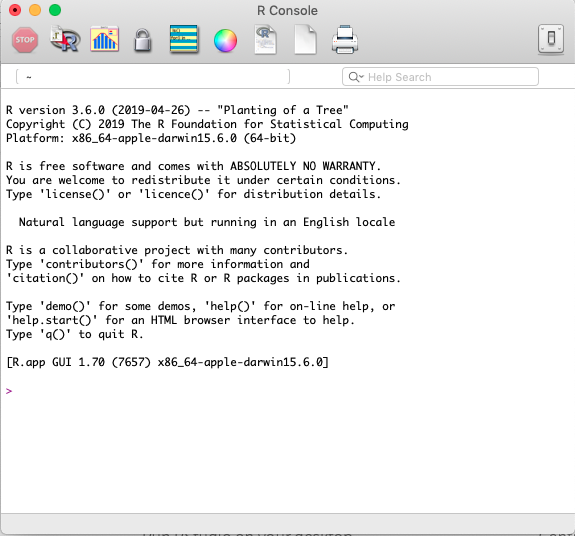
\includegraphics{atlas/r_screenshot.png}

This looks a bit intimidating, but you'll almost never open R directly and interact with it in that way.

To analyse data with R, you will typically write out a text file containing your code. This file - which we'll call a script - should be able to be read and executed by R from start to finish. The easiest way to write your code, run your script, and generate your outputs (whether that's a chart, a document, or a set of model results) is to use RStudio.

\hypertarget{what-is-rstudio}{%
\section{What is RStudio?}\label{what-is-rstudio}}

RStudio is another piece of free software you can download and run on your computer.\footnote{RStudio is, somewhat confusingly, a product made by a company called RStudio. Although the RStudio desktop software is free, RStudio makes money by charging for other services, like running R in the cloud. When we refer to RStudio, we're referring to the desktop software unless we make it clear that we mean the company.} It's also available for Windows, macOS and Linux. In programmer jargon, RStudio is an ``integrated development environment'' or IDE. This means RStudio has a range of tools that help you work with R. It has a text editor for you to write R scripts, an R `console' to interact directly with the language, and panes that let you see the objects you have stored in memory and any graphs you've created.

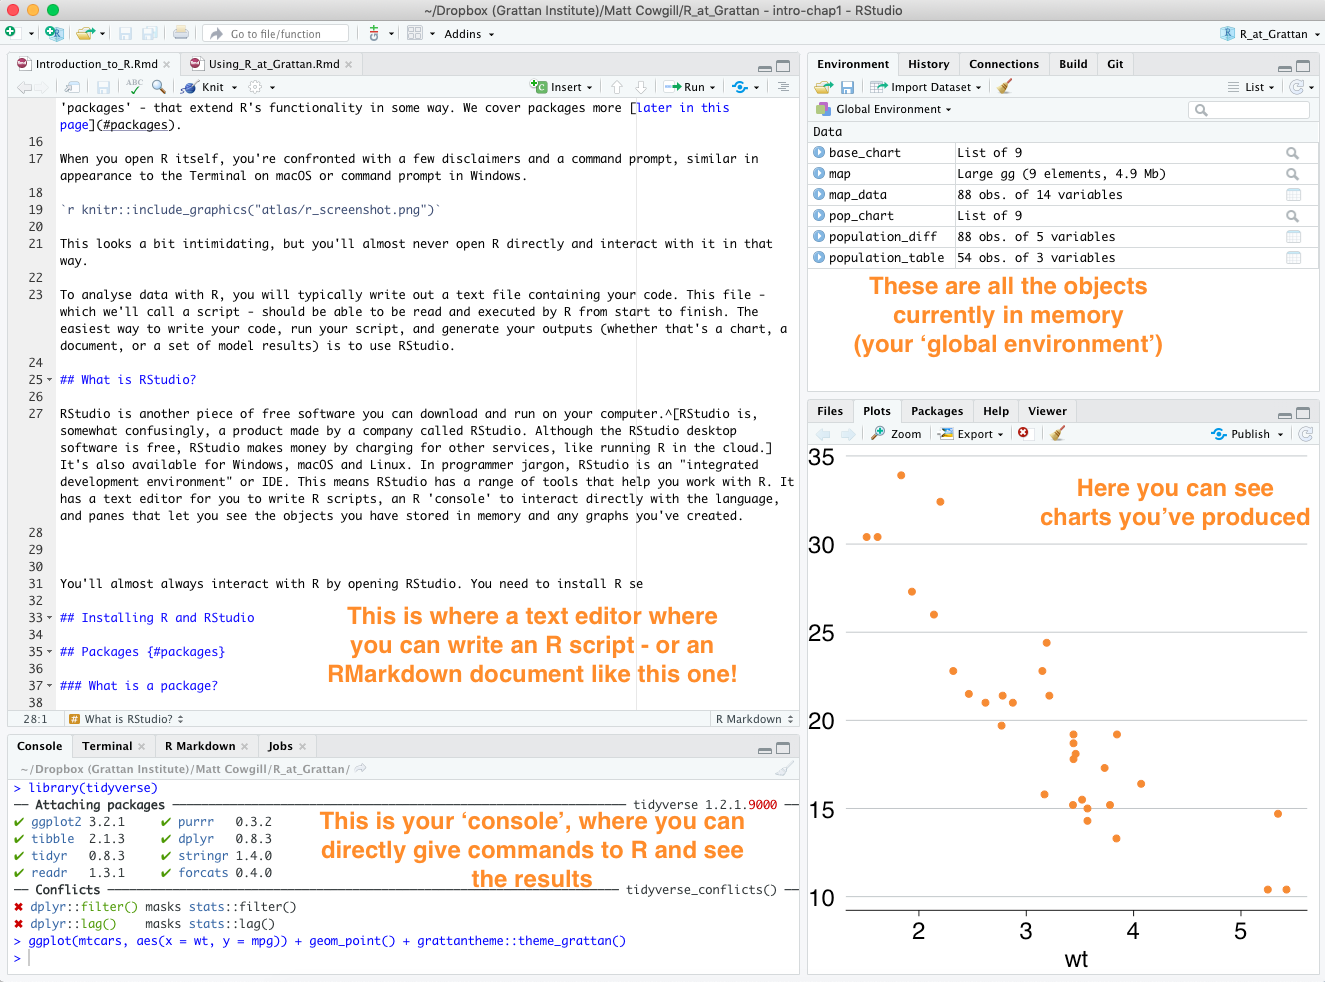
\includegraphics{atlas/rstudio_screenshot.png}

You'll almost always interact with R by opening RStudio.

\hypertarget{installing-r-and-rstudio}{%
\section{Installing R and RStudio}\label{installing-r-and-rstudio}}

Although you'll usually work with R by opening RStudio, you need to install both R and RStudio separately.

Install R by going to \href{https://cran.r-project.org}{CRAN}, the Comprehensive R Archive Network. CRAN is a community-run website that houses R itself as well as a broad range of R packages.

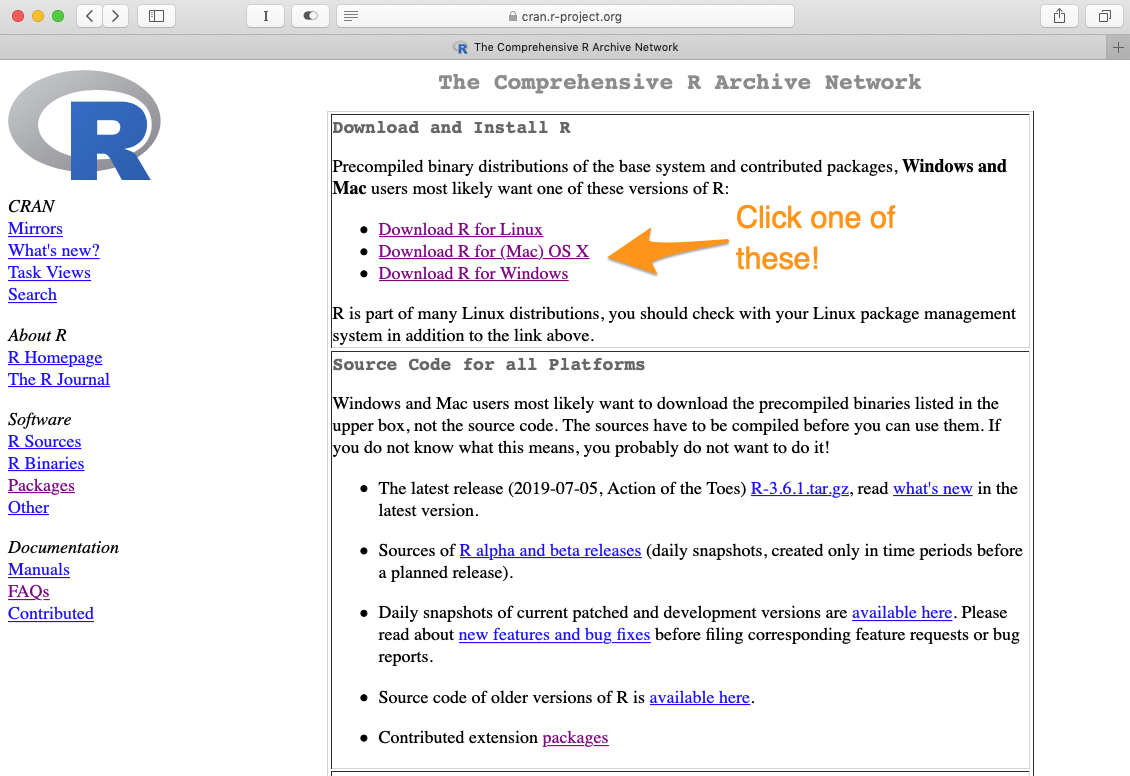
\includegraphics{atlas/r_cran.png}

You want to download the latest base R release, as a `binary'. Don't worry, you don't need to know what a binary is.

For macOS, the page will look like this:
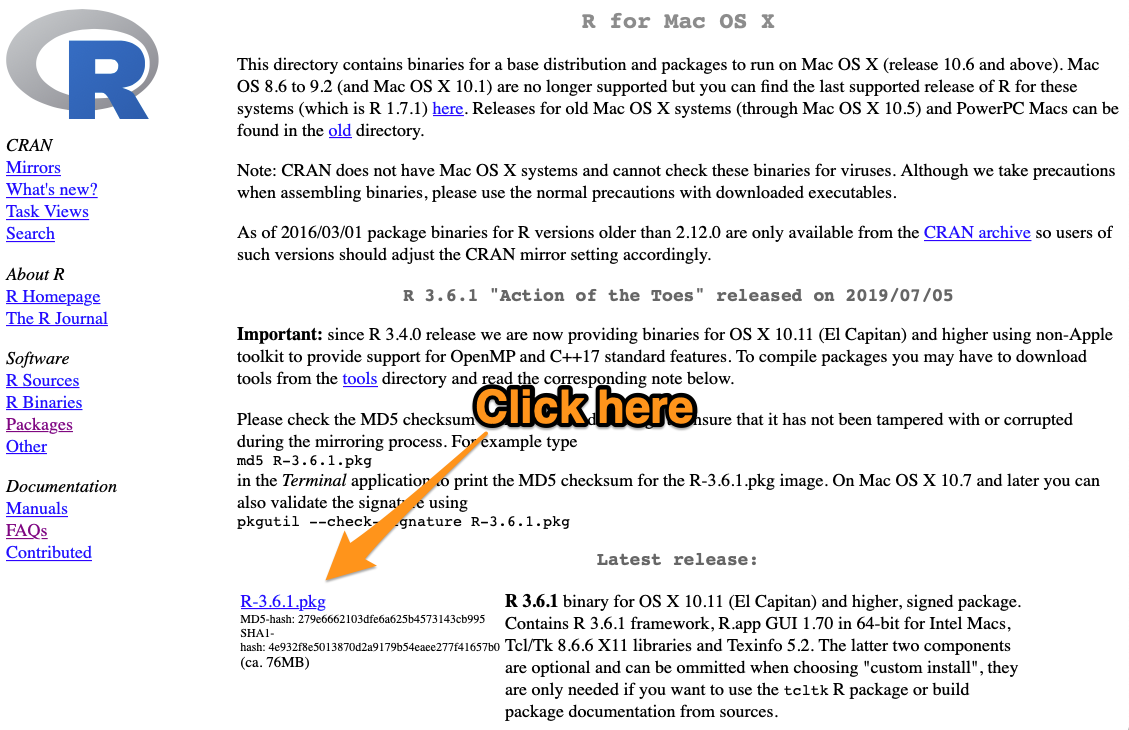
\includegraphics{atlas/r_cran_macos.png}

For Windows, you'll need to click on the `base' version, and then click again to start the download.

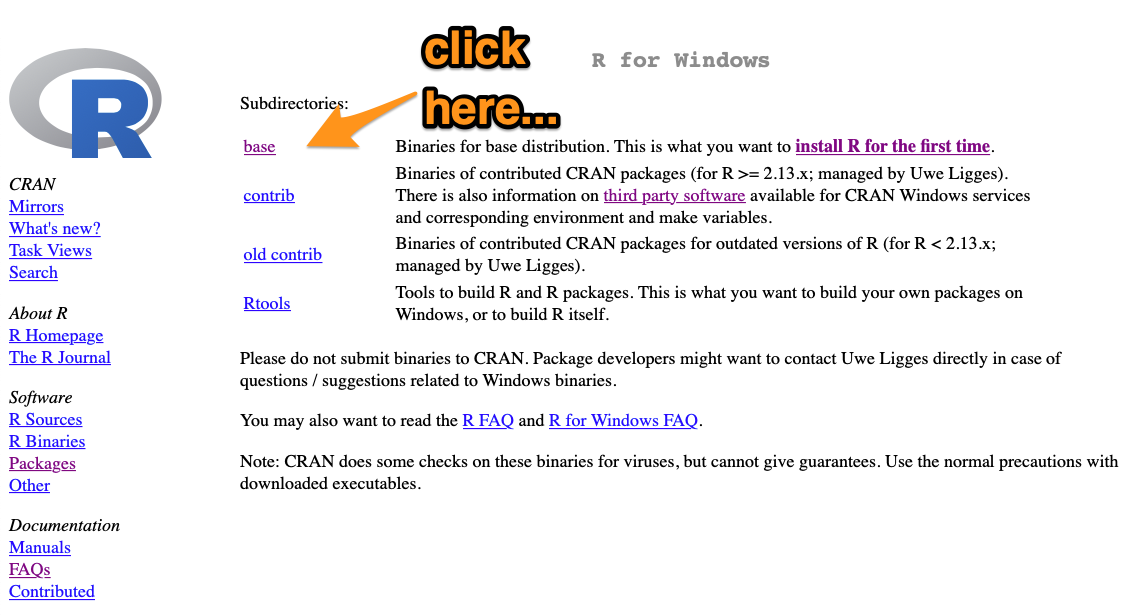
\includegraphics{atlas/r_cran_windows_1.png} 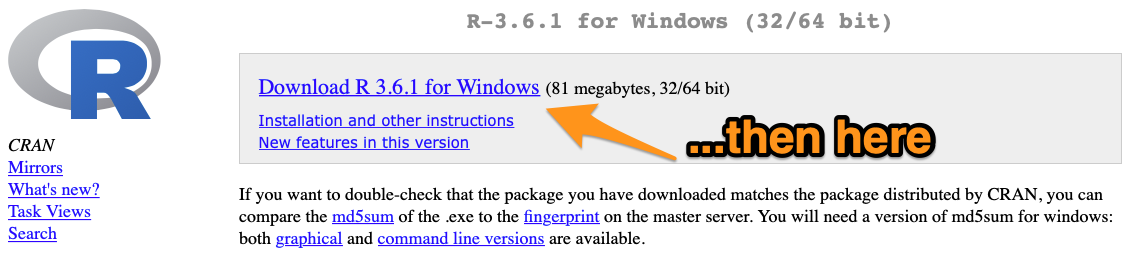
\includegraphics{atlas/r_cran_windows_2.png}

Once you've installed R, you'll need to install RStudio. Go to the \href{https://www.rstudio.com/products/rstudio/download/\#download}{RStudio website and install the latest version} of RStudio Desktop (open source license).

Once they're both installed, get started by opening RStudio.

\hypertarget{packages}{%
\section{Packages}\label{packages}}

R comes with a lot of functions - commands - built in to do a broad range of data tasks. You could, if you really wanted, import a dataset, clean it up, estimate a model, and make a plot all using the functions that come with R - known as `base R'\footnote{Technically some of the `built-in' functions are part of packages, like the \texttt{tools}, \texttt{utils} and \texttt{stats} packages that come with R. We'll refer to all these as base R.}.

But a lot of our work at Grattan uses add-on software to base R, known as `packages'. Some packages, like the popular `dplyr', make it quicker and/or easier to do tasks that you could otherwise do in base R. Other packages expand the possibilities of what R can do - like fitting a machine learning model, for example.

Like R itself, packages are free and open source. You can install them from within RStudio.

At Grattan, we make heavy use of a set of related packages known collectively as the \texttt{tidyverse}. We'll cover these more in a later chapter.

\hypertarget{installing-packages}{%
\subsection{Installing packages}\label{installing-packages}}

You'll typically install packages using the console in RStudio. That's the part of the window that, by default, sits in the bottom-left corner of the screen.

In our work at Grattan, we use packages from two different source: CRAN and Github. The main difference you need to know about is that we use different commands to install packages from these two sources.

To install a package from CRAN, we use the command \texttt{install.packages()}.

For example, this code will install the \texttt{ggplot2} package from CRAN:

\begin{Shaded}
\begin{Highlighting}[]
\KeywordTok{install.packages}\NormalTok{(}\StringTok{"ggplot2"}\NormalTok{)}
\end{Highlighting}
\end{Shaded}

To install a package from Github, we use the function \texttt{install\_github()}. Unfortunately, this package doesn't come with R - it's part of the \texttt{devtools} package. First, we install devtools from CRAN:

\begin{Shaded}
\begin{Highlighting}[]
\KeywordTok{install.packages}\NormalTok{(}\StringTok{"devtools"}\NormalTok{)}
\end{Highlighting}
\end{Shaded}

Now we can install packages from Github using the \texttt{install\_github()} function from the \texttt{devtools} package. For example, here's how we would install the Grattan ggplot2 theme, which we'll discuss later in this website:

\begin{Shaded}
\begin{Highlighting}[]
\NormalTok{devtools}\OperatorTok{::}\KeywordTok{install_github}\NormalTok{(}\StringTok{"mattcowgill/grattantheme"}\NormalTok{, }\DataTypeTok{dependencies =} \OtherTok{TRUE}\NormalTok{)}
\end{Highlighting}
\end{Shaded}

\hypertarget{using-packages}{%
\subsection{Using packages}\label{using-packages}}

Before using a function that comes from a package, as opposed to base R, you need to tell R where to look for the function. There are two main ways to do that.

We can either load (aka `attach') the package by using the \texttt{library()} function:

\begin{Shaded}
\begin{Highlighting}[]
\KeywordTok{library}\NormalTok{(devtools)}

\CommentTok{# Now that the `devtools` package is loaded, we can use its `install_github()` function:}

\KeywordTok{install_github}\NormalTok{(}\StringTok{"mattcowgill/grattantheme"}\NormalTok{)}
\end{Highlighting}
\end{Shaded}

Or, we can use two colons - \texttt{::} - to tell R to use an individual function from a package without loading it:

\begin{Shaded}
\begin{Highlighting}[]
\NormalTok{devtools}\OperatorTok{::}\KeywordTok{install_github}\NormalTok{(}\StringTok{"mattcowgill/grattantheme"}\NormalTok{)}
\end{Highlighting}
\end{Shaded}

It usually makes sense to load a package with \texttt{library()}, unless you only need to use one of its function once or twice. There's no harm to using the \texttt{::} operator even if you have already loaded a package with \texttt{library()}. This can remove ambiguity both for R and for humans reading your code, particularly if you're using an obscure function - it makes it clearer where the function comes from.

\hypertarget{why-use-r}{%
\chapter{Why use R?}\label{why-use-r}}

We can break this question into two parts:
1. Why use script-based software to analyse data?
2. Why use R, specifically?

\hypertarget{why-script}{%
\section{Why use script-based software?}\label{why-script}}

\begin{enumerate}
\def\labelenumi{\arabic{enumi}.}
\tightlist
\item
  Make your analysis reproducible by setting out the complete series of steps taken from raw data to final output.
\item
  Work with large data sets.
\end{enumerate}

\hypertarget{why-R}{%
\section{Why use R specifically?}\label{why-R}}

\begin{Shaded}
\begin{Highlighting}[]
\KeywordTok{library}\NormalTok{(tidyverse)}
\end{Highlighting}
\end{Shaded}

\hypertarget{intro}{%
\chapter{Using R at Grattan}\label{intro}}

\hypertarget{using-r-projects-for-a-fully-reproducible-workflow.}{%
\section{Using R projects for a fully reproducible workflow.}\label{using-r-projects-for-a-fully-reproducible-workflow.}}

\emph{Finally adhering to the `hit by a bus' rule.}

Having a clear, consistent structure for our analyses means that our work is more easily checked and revised, including by ourselves in the future. A small investment of time up front to set up your analysis will save time (your own and others') down the track.

Cover:
1. setwd() and machine-speficic filepaths are bad
2. relative file paths are good
3. RStudio projects are an easy, reproducible way to set your wd

\hypertarget{filepaths}{%
\subsection{Filepaths}\label{filepaths}}

Filepaths should be relative to the working directory, and the working directory should be set by the project.

\textbf{Good}

\begin{Shaded}
\begin{Highlighting}[]
\NormalTok{hes <-}\StringTok{ }\KeywordTok{read_csv}\NormalTok{(}\StringTok{"data/HES/hes1516.csv"}\NormalTok{)}
\KeywordTok{grattan_save}\NormalTok{(}\StringTok{"images/expenditure_by_income.pdf"}\NormalTok{)}
\end{Highlighting}
\end{Shaded}

\textbf{Bad}

\begin{Shaded}
\begin{Highlighting}[]
\NormalTok{hes <-}\StringTok{ }\KeywordTok{read_csv}\NormalTok{(}\StringTok{"/Users/mcowgill/Desktop/hes1516.csv"}\NormalTok{)}
\NormalTok{hes <-}\StringTok{ }\KeywordTok{read_csb}\NormalTok{(}\StringTok{"C:\textbackslash{}Users\textbackslash{}mcowgill\textbackslash{}Desktop\textbackslash{}hes1516.csv"}\NormalTok{)}
\KeywordTok{grattan_save}\NormalTok{(}\StringTok{"/Users/mcowgill/Desktop/images/expenditure_by_income.pdf"}\NormalTok{)}
\end{Highlighting}
\end{Shaded}

\hypertarget{keep-your-scripts-manageable}{%
\subsection{Keep your scripts manageable}\label{keep-your-scripts-manageable}}

As a general rule of thumb, use one script per output. It should be clear what your script is trying to do (use comments!).

Consider breaking your analysis into pieces. For example:

\begin{itemize}
\tightlist
\item
  01\_import.R
\item
  02\_tidy.R
\item
  03\_model.R
\item
  04\_visualise.R
\end{itemize}

\textbf{Don't} include interactive work (like \texttt{View(mydf)}, \texttt{str(mydf)}, \texttt{mean(mydf\$variable)}, etc.) in your saved script.

\hypertarget{use-subfolders-of-your-project-folder}{%
\subsection{Use subfolders of your project folder}\label{use-subfolders-of-your-project-folder}}

Remember the hit-by-a-bus rule. It should be easy for any Grattan colleague to open your project folder and get up to speed with what it does. Putting all your files - raw data, scripts, output - in the one folder makes it harder to understand how your work fits together.

Use subfolders to clearly separate your code, raw data, and output.

\hypertarget{grattan-coding-style-guide}{%
\section{Grattan coding style guide}\label{grattan-coding-style-guide}}

Short summary of why

Link to style guide

\hypertarget{what-is-the-tidyverse-and-why-do-we-use-it}{%
\section{What is the tidyverse and why do we use it?}\label{what-is-the-tidyverse-and-why-do-we-use-it}}

Introduce following chapters

\hypertarget{an-introduction-to-rmarkdown}{%
\section{An introduction to RMarkdown}\label{an-introduction-to-rmarkdown}}

\hypertarget{resources-in-this-package}{%
\section{Resources in this package}\label{resources-in-this-package}}

\begin{itemize}
\tightlist
\item
  Starting a piece of analysis `cheat sheet'.
\item
  Updated style guide.
\item
  Written guide/slides.
\end{itemize}

\hypertarget{data-visualisation}{%
\chapter{Data Visualisation}\label{data-visualisation}}

{[}intro{]}

\hypertarget{set-up-and-packages}{%
\section{Set-up and packages}\label{set-up-and-packages}}

This section uses the package \texttt{ggplot2} to visualise data, and \texttt{dplyr} functions to manipulate data. Both of these packages are loaded with \texttt{tidyverse}. The \texttt{scales} package helps with labelling your axes.

The \texttt{grattantheme} package is used to make charts look Grattan-y. The \texttt{absmapsdata} package is used to help make maps.

\begin{Shaded}
\begin{Highlighting}[]
\KeywordTok{library}\NormalTok{(tidyverse)}
\KeywordTok{library}\NormalTok{(grattantheme)}
\KeywordTok{library}\NormalTok{(absmapsdata)}
\KeywordTok{library}\NormalTok{(sf)}
\KeywordTok{library}\NormalTok{(scales)}
\end{Highlighting}
\end{Shaded}

For most charts in this chapter, we'll use the \texttt{population\_table} data summarised here. It contains the population in each state between 2013 and 2018:

\begin{Shaded}
\begin{Highlighting}[]
\NormalTok{population_table <-}\StringTok{ }\KeywordTok{read_csv}\NormalTok{(}\StringTok{"data/population_sa4.csv"}\NormalTok{) }\OperatorTok\StringTok{ }
\StringTok{        }\KeywordTok{filter}\NormalTok{(data_item }\OperatorTok{==}\StringTok{ "Persons - Total (no.)"}\NormalTok{) }\OperatorTok\StringTok{ }
\StringTok{        }\KeywordTok{mutate}\NormalTok{(}\DataTypeTok{pop =} \KeywordTok{as.numeric}\NormalTok{(value),}
               \DataTypeTok{year =} \KeywordTok{as.factor}\NormalTok{(year)) }\OperatorTok\StringTok{ }
\StringTok{        }\KeywordTok{group_by}\NormalTok{(year, state) }\OperatorTok\StringTok{ }
\StringTok{        }\KeywordTok{summarise}\NormalTok{(}\DataTypeTok{pop =} \KeywordTok{sum}\NormalTok{(pop))}

\CommentTok{# Show the first six rows of the new dataset}
\KeywordTok{head}\NormalTok{(population_table)}
\end{Highlighting}
\end{Shaded}

\begin{verbatim}
## # A tibble: 6 x 3
## # Groups:   year [1]
##   year  state                            pop
##   <fct> <chr>                          <dbl>
## 1 2013  Australian Capital Territory  383257
## 2 2013  New South Wales              7404032
## 3 2013  Northern Territory            241722
## 4 2013  Other Territories               2962
## 5 2013  Queensland                   4652824
## 6 2013  South Australia              1671488
\end{verbatim}

\hypertarget{concepts}{%
\section{Concepts}\label{concepts}}

The \texttt{ggplot2} package is based on the \texttt{g}rammar of \texttt{g}raphics. \ldots{}

The main ingredients to a \texttt{ggplot} chart:

\begin{itemize}
\tightlist
\item
  \textbf{Data}: what data should be plotted. e.g. \texttt{data}
\item
  \textbf{Aesthetics}: what variables should be linked to what chart elements. e.g. \texttt{aes(x\ =\ population,\ y\ =\ age)} to connect the \texttt{population} variable to the \texttt{x} axis, and the \texttt{age} variable to the \texttt{y} axis.
\item
  \textbf{Geoms}: how the data should be plotted. e.g. \texttt{geom\_point()} will produce a scatter plot, \texttt{geom\_col} will produce a column chart.
\end{itemize}

Each plot you make will be made up of these three elements. The \href{https://ggplot2.tidyverse.org/reference/}{full list of standard geoms} is listed in the \texttt{tidyverse} documentation.

\begin{Shaded}
\begin{Highlighting}[]
\KeywordTok{ggplot}\NormalTok{(}\DataTypeTok{data =} \OperatorTok{<}\NormalTok{DATA}\OperatorTok{>}\NormalTok{) }\OperatorTok{+}\StringTok{ }
\StringTok{  }\ErrorTok{<}\NormalTok{GEOM_FUNCTION}\OperatorTok{>}\NormalTok{(}
     \DataTypeTok{mapping =} \KeywordTok{aes}\NormalTok{(}\OperatorTok{<}\NormalTok{MAPPINGS}\OperatorTok{>}\NormalTok{),}
     \DataTypeTok{stat =} \OperatorTok{<}\NormalTok{STAT}\OperatorTok{>}\NormalTok{, }
     \DataTypeTok{position =} \OperatorTok{<}\NormalTok{POSITION}\OperatorTok{>}
\StringTok{  }\NormalTok{) }\OperatorTok{+}
\StringTok{  }\ErrorTok{<}\NormalTok{COORDINATE_FUNCTION}\OperatorTok{>}\StringTok{ }\OperatorTok{+}
\StringTok{  }\ErrorTok{<}\NormalTok{FACET_FUNCTION}\OperatorTok{>}
\end{Highlighting}
\end{Shaded}

For example, you can plot a column chart by passing the \texttt{population\_table} dataset into \texttt{ggplot()} (``make a chart wth this data''). This produces an empty plot:

\begin{Shaded}
\begin{Highlighting}[]
\NormalTok{population_table }\OperatorTok\StringTok{ }
\StringTok{        }\KeywordTok{ggplot}\NormalTok{()}
\end{Highlighting}
\end{Shaded}


\includegraphics{Data_visualisation_files/figure-latex/empty plot-1.pdf}

Next, set the \texttt{aes} (aesthetics) to \texttt{x\ =\ state} (``make the x-axis represent state''), \texttt{y\ =\ pop} (``the y-axis should represent population''), and \texttt{fill\ =\ year} (``the fill colour represents year''). Now \texttt{ggplot} knows where things should \emph{go}:\texttt{\{r\ empty\ with\ aes\}\ population\_table\ \%\textgreater{}\%\ \ \ \ \ \ \ \ \ \ ggplot(aes(x\ =\ state,\ \ \ \ \ \ \ \ \ \ \ \ \ \ \ \ \ \ \ \ y\ =\ pop,\ \ \ \ \ \ \ \ \ \ \ \ \ \ \ \ \ \ \ \ fill\ =\ year))}

Now that \texttt{ggplot} knows where things should go, it needs to \emph{how} to plot them. For this we use \texttt{geoms}. Tell it to plot a column chart by using \texttt{geom\_col}:

\begin{Shaded}
\begin{Highlighting}[]
\NormalTok{population_table }\OperatorTok\StringTok{ }
\StringTok{        }\KeywordTok{ggplot}\NormalTok{(}\KeywordTok{aes}\NormalTok{(}\DataTypeTok{x =}\NormalTok{ state,}
                   \DataTypeTok{y =}\NormalTok{ pop,}
                   \DataTypeTok{fill =}\NormalTok{ year)) }\OperatorTok{+}
\StringTok{        }\KeywordTok{geom_col}\NormalTok{()}
\end{Highlighting}
\end{Shaded}

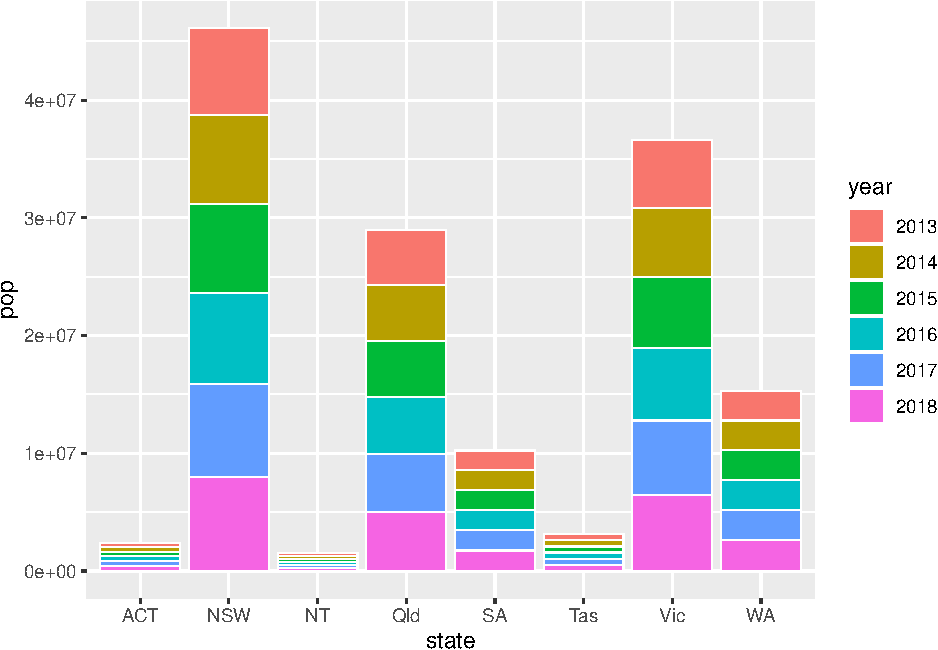
\includegraphics{Data_visualisation_files/figure-latex/complete plot-1.pdf}

Great! Although stacking populations is a bit silly. You can adjust the way \texttt{geoms} work with arguments. In this case, tell it to place the different categories next to each other rather than ontop of each other using \texttt{position\ =\ "dodge"}:

\begin{Shaded}
\begin{Highlighting}[]
\NormalTok{population_table }\OperatorTok\StringTok{ }
\StringTok{        }\KeywordTok{ggplot}\NormalTok{(}\KeywordTok{aes}\NormalTok{(}\DataTypeTok{x =}\NormalTok{ state,}
                   \DataTypeTok{y =}\NormalTok{ pop,}
                   \DataTypeTok{fill =}\NormalTok{ year)) }\OperatorTok{+}
\StringTok{        }\KeywordTok{geom_col}\NormalTok{(}\DataTypeTok{position =} \StringTok{"dodge"}\NormalTok{)}
\end{Highlighting}
\end{Shaded}

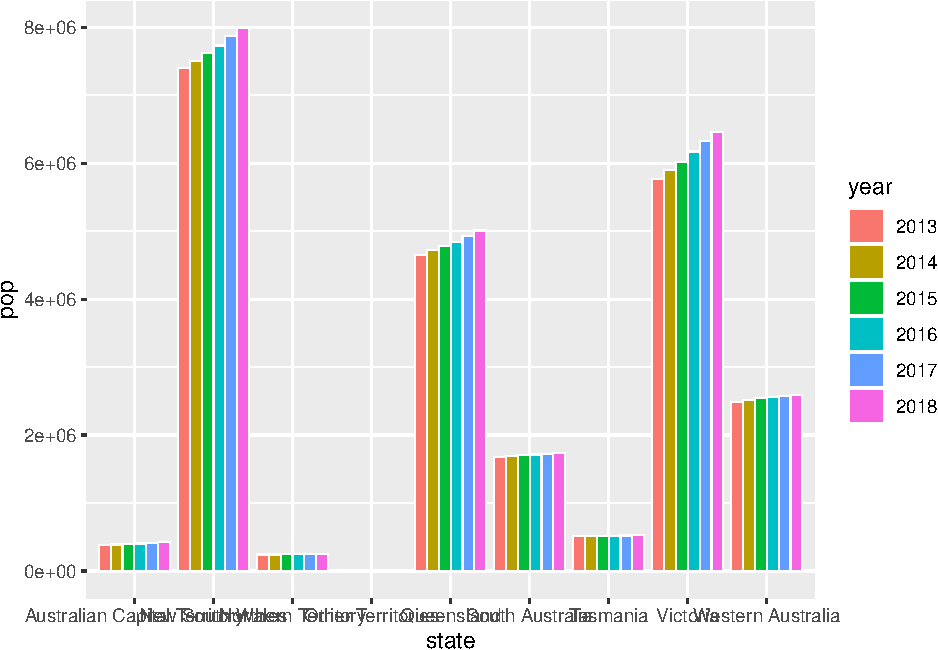
\includegraphics{Data_visualisation_files/figure-latex/with dodge-1.pdf}

That's nicer. The following sections in this chapter will build on this chart. The rest of the chapter will explore:

\begin{itemize}
\tightlist
\item
  Grattanising your charts and choosing colours
\item
  Saving charts according to Grattan templates
\item
  Making bar, line, scatter and distribution plots
\item
  Making maps and interactive charts
\item
  Adding chart labels
\end{itemize}

\hypertarget{making-grattan-y-charts}{%
\section{Making Grattan-y charts}\label{making-grattan-y-charts}}

The \texttt{grattantheme} package contains functions that help \emph{Grattanise} your charts. It is hosted here: \url{https://github.com/mattcowgill/grattantheme}

You can install it with \texttt{devtools::install\_github} from the package:

\begin{Shaded}
\begin{Highlighting}[]
\KeywordTok{install.packages}\NormalTok{(}\StringTok{"devtools"}\NormalTok{)}
\NormalTok{remotes}\OperatorTok{::}\KeywordTok{install_github}\NormalTok{(}\StringTok{"mattcowgill/grattantheme"}\NormalTok{)}
\end{Highlighting}
\end{Shaded}

The key functions of \texttt{grattantheme} are:

\begin{itemize}
\tightlist
\item
  \texttt{theme\_grattan}: set size, font and colour defaults that adhere to the Grattan style guide.
\item
  \texttt{grattan\_y\_continuous}: sets the right defaults for a continuous y-axis.
\item
  \texttt{grattan\_colour\_continuous}: pulls colours from the Grattan colour palete for \texttt{colour} aesthetics.
\item
  \texttt{grattan\_fill\_continuous}: pulls colours from the Grattan colour palete for \texttt{fill} aesthetics.
\item
  \texttt{grattan\_save}: a save function that exports charts in correct report or presentation dimensions.
\end{itemize}

This section will run through some examples of \emph{Grattanising} charts. The \texttt{ggplot} functions are explored in more detail in the next section.

\hypertarget{making-grattan-charts}{%
\subsection{Making Grattan charts}\label{making-grattan-charts}}

Start with a column chart, similar to the one made above:

\begin{Shaded}
\begin{Highlighting}[]
\NormalTok{base_chart <-}\StringTok{ }\NormalTok{population_table }\OperatorTok\StringTok{ }
\StringTok{        }\KeywordTok{ggplot}\NormalTok{(}\KeywordTok{aes}\NormalTok{(}\DataTypeTok{x =}\NormalTok{ state,}
                   \DataTypeTok{y =}\NormalTok{ pop,}
                   \DataTypeTok{fill =}\NormalTok{ year)) }\OperatorTok{+}
\StringTok{        }\KeywordTok{geom_col}\NormalTok{(}\DataTypeTok{position =} \StringTok{"dodge"}\NormalTok{) }\OperatorTok{+}
\StringTok{        }\KeywordTok{labs}\NormalTok{(}\DataTypeTok{x =} \StringTok{""}\NormalTok{,}
             \DataTypeTok{title =} \StringTok{"NSW and Victoria are booming"}\NormalTok{,}
             \DataTypeTok{subtitle =} \StringTok{"Population by state, 2013-2018"}\NormalTok{,}
             \DataTypeTok{caption =} \StringTok{"Source: ABS Regional Dataset (2019)"}\NormalTok{)}

\NormalTok{base_chart}
\end{Highlighting}
\end{Shaded}

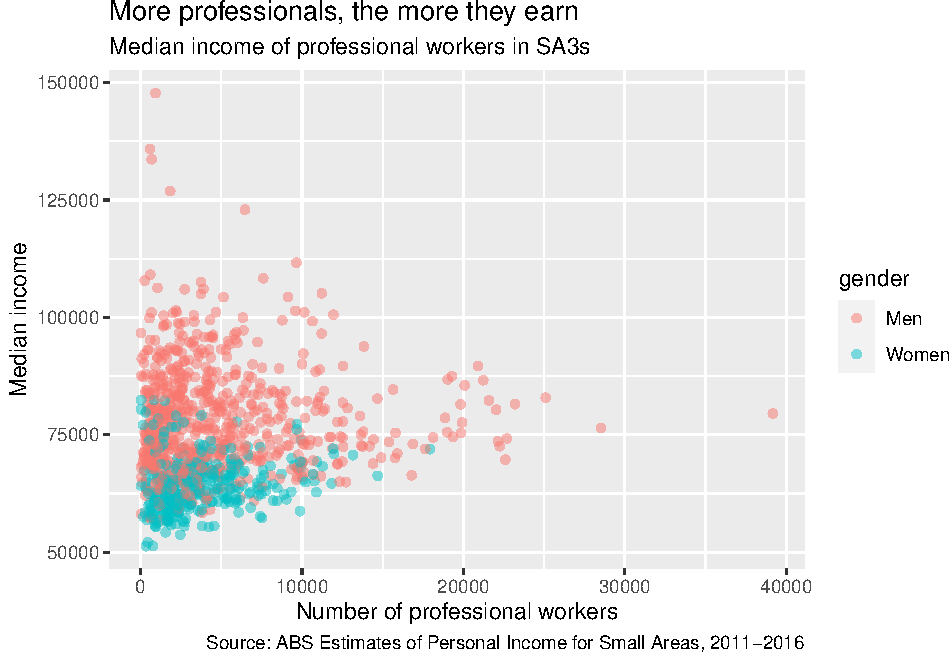
\includegraphics{Data_visualisation_files/figure-latex/base_chart-1.pdf}

Let's make it Grattany. First, add \texttt{theme\_grattan} to your plot:

\begin{Shaded}
\begin{Highlighting}[]
\NormalTok{base_chart }\OperatorTok{+}
\StringTok{        }\KeywordTok{theme_grattan}\NormalTok{()}
\end{Highlighting}
\end{Shaded}

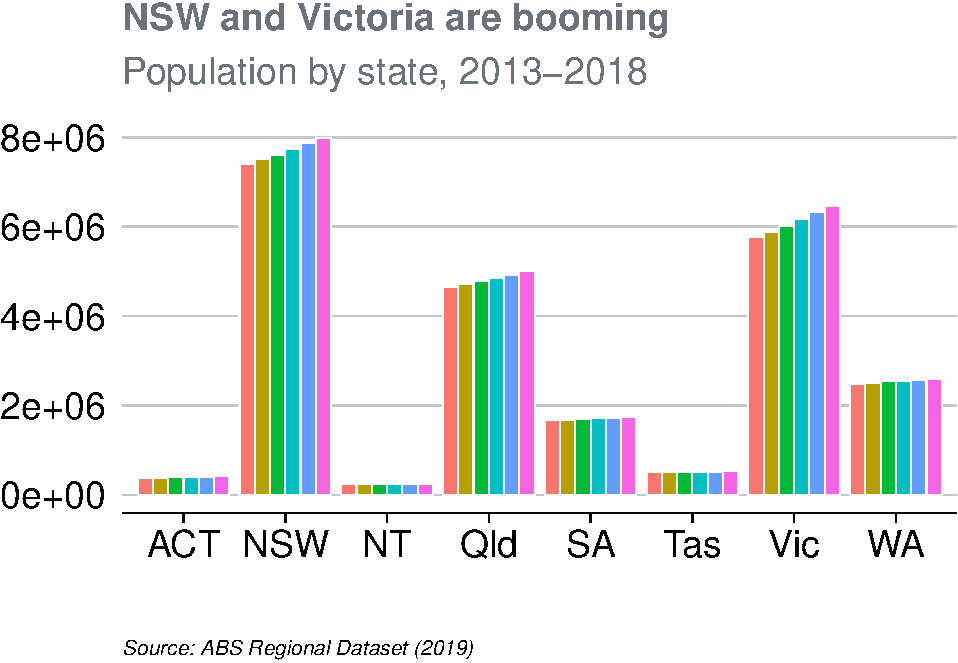
\includegraphics{Data_visualisation_files/figure-latex/add_theme_grattan-1.pdf}

Then \texttt{grattan\_y\_continuous} to align the x-axis with zero. This function takes the same arguments as \texttt{scale\_y\_continuous}, so you can add \texttt{labels\ =\ comma()} to reformat the y-axis labels:

\begin{Shaded}
\begin{Highlighting}[]
\NormalTok{base_chart }\OperatorTok{+}
\StringTok{        }\KeywordTok{theme_grattan}\NormalTok{() }\OperatorTok{+}
\StringTok{        }\KeywordTok{grattan_y_continuous}\NormalTok{(}\DataTypeTok{labels =}\NormalTok{ comma)}
\end{Highlighting}
\end{Shaded}

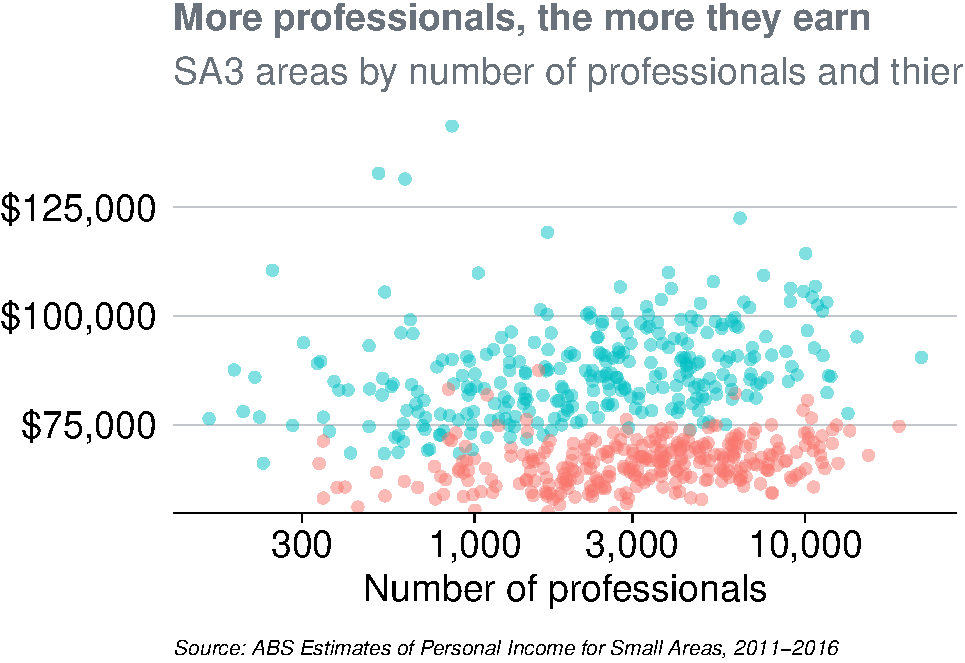
\includegraphics{Data_visualisation_files/figure-latex/add_grattan_y_continuous-1.pdf}

To define \texttt{fill} colours, use \texttt{grattan\_fill\_manual} with the number of colours you need (six, in this case):

\begin{Shaded}
\begin{Highlighting}[]
\NormalTok{pop_chart <-}\StringTok{ }\NormalTok{base_chart }\OperatorTok{+}
\StringTok{        }\KeywordTok{theme_grattan}\NormalTok{() }\OperatorTok{+}
\StringTok{        }\KeywordTok{grattan_y_continuous}\NormalTok{(}\DataTypeTok{labels =}\NormalTok{ comma) }\OperatorTok{+}
\StringTok{        }\KeywordTok{grattan_fill_manual}\NormalTok{(}\DecValTok{6}\NormalTok{)}

\NormalTok{pop_chart}
\end{Highlighting}
\end{Shaded}

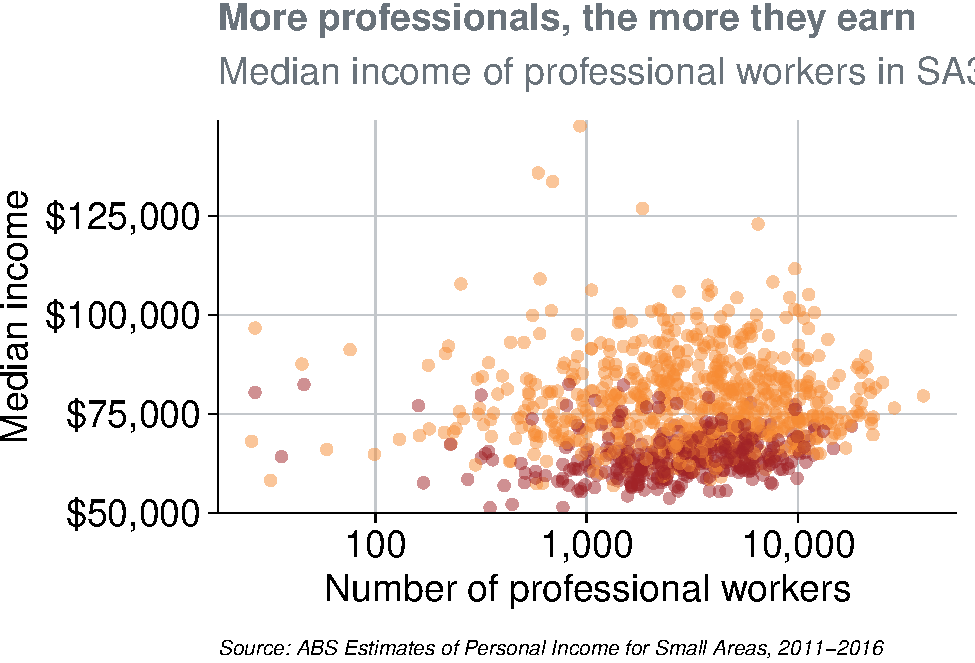
\includegraphics{Data_visualisation_files/figure-latex/add_fill-1.pdf}

Nice chart! Now you can save it and share it with the world.

\hypertarget{saving-grattan-charts}{%
\subsection{Saving Grattan charts}\label{saving-grattan-charts}}

The \texttt{grattan\_save} function saves your charts according to Grattan templates. It takes these arguments:

\begin{itemize}
\tightlist
\item
  \texttt{filename}: the path, name and file-type of your saved chart. eg: \texttt{"atlas/population\_chart.pdf"}.
\item
  \texttt{object}: the R object that you want to save. eg: \texttt{pop\_chart}. If left blank, it grabs the last chart that was displayed.
\item
  \texttt{type}: the Grattan template to be used. This is one of:

  \begin{itemize}
  \tightlist
  \item
    \texttt{"normal"} The default. Use for normal Grattan report charts, or to paste into a 4:3 Powerpoint slide. Width: 22.2cm, height: 14.5cm.
  \item
    \texttt{"normal\_169"} Only useful for pasting into a 16:9 format Grattan Powerpoint slide. Width: 30cm, height: 14.5cm.
  \item
    \texttt{"tiny"} Fills the width of a column in a Grattan report, but is shorter than usual. Width: 22.2cm, height: 11.1cm.
  \item
    \texttt{"wholecolumn"} Takes up a whole column in a Grattan report. Width: 22.2cm, height: 22.2cm.
  \item
    \texttt{"fullpage"} Fills a whole page of a Grattan report. Width: 44.3cm, height: 22.2cm.
  \item
    \texttt{"fullslide"} Creates an image that looks like a 4:3 Grattan Powerpoint slide, complete with logo. Width: 25.4cm, height: 19.0cm.
  \item
    \texttt{"fullslide\_169"} Creates` an image that looks like a 16:9 Grattan Powerpoint slide, complete with logo. Use this to drop into standard presentations. Width: 33.9cm, height: 19.0cm
  \item
    \texttt{"blog"} Creates a 4:3 image that looks like a Grattan Powerpoint slide, but with less border whitespace than `fullslide'."
  \item
    \texttt{"fullslide\_44"\ Creates} an image that looks like a 4:4 Grattan Powerpoint slide. This may be useful for taller charts for the Grattan blog; not useful for any other purpose. Width: 25.4cm, height: 25.4cm.
  \item
    Set \texttt{type\ =\ "all"} to save your chart in all available sizes.
  \end{itemize}
\item
  \texttt{height}: override the height set by \texttt{type}. This can be useful for really long charts in blogposts.
\item
  \texttt{save\_data}: exports a \texttt{csv} file containing the data used in the chart.
\item
  \texttt{force\_labs}: override the removal of labels for a particular \texttt{type}. eg \texttt{force\_labs\ =\ TRUE} will keep the y-axis label.
\end{itemize}

To save the \texttt{pop\_chart} plot created above as a whole-column chart for a \textbf{report}:

\begin{Shaded}
\begin{Highlighting}[]
\KeywordTok{grattan_save}\NormalTok{(}\StringTok{"atlas/population_chart_report.pdf"}\NormalTok{, pop_chart, }\DataTypeTok{type =} \StringTok{"wholecolumn"}\NormalTok{)}
\end{Highlighting}
\end{Shaded}

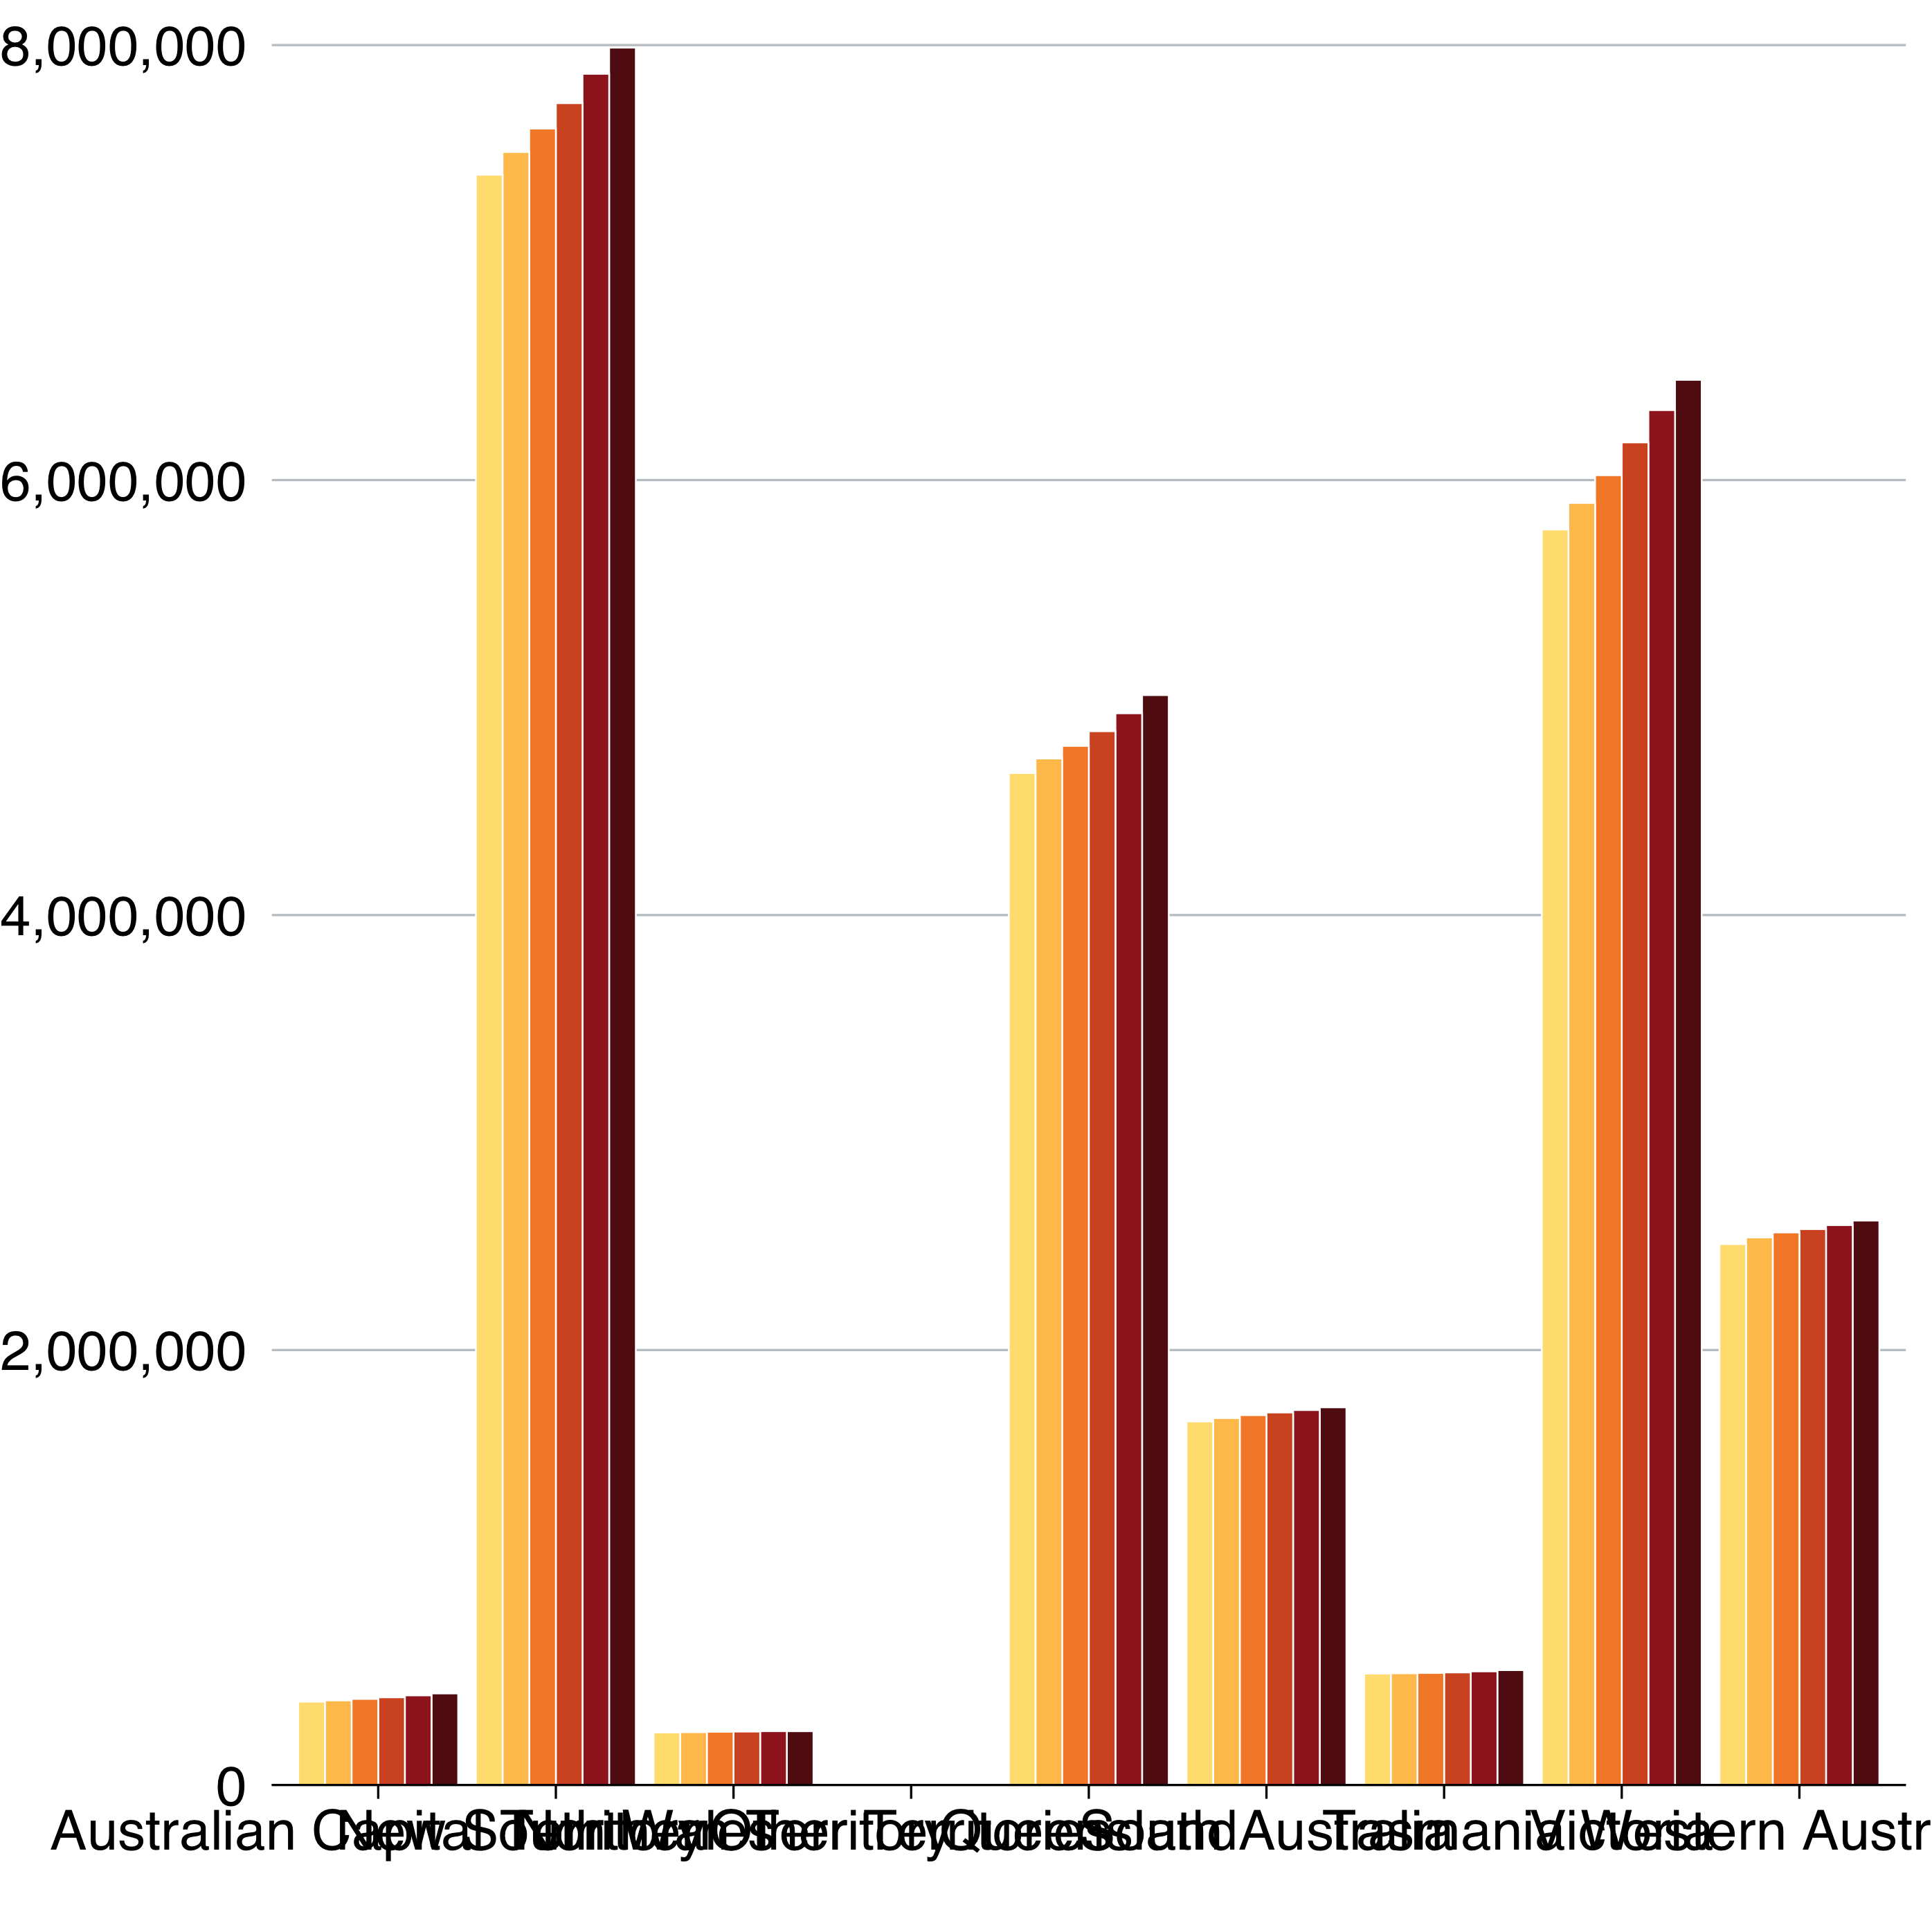
\includegraphics{atlas/population_chart_report.png}

To save it as a \textbf{presentation} slide instead, use \texttt{type\ =\ "fullslide"}:

\begin{Shaded}
\begin{Highlighting}[]
\KeywordTok{grattan_save}\NormalTok{(}\StringTok{"atlas/population_chart_presentation.pdf"}\NormalTok{, pop_chart, }\DataTypeTok{type =} \StringTok{"fullslide"}\NormalTok{)}
\end{Highlighting}
\end{Shaded}

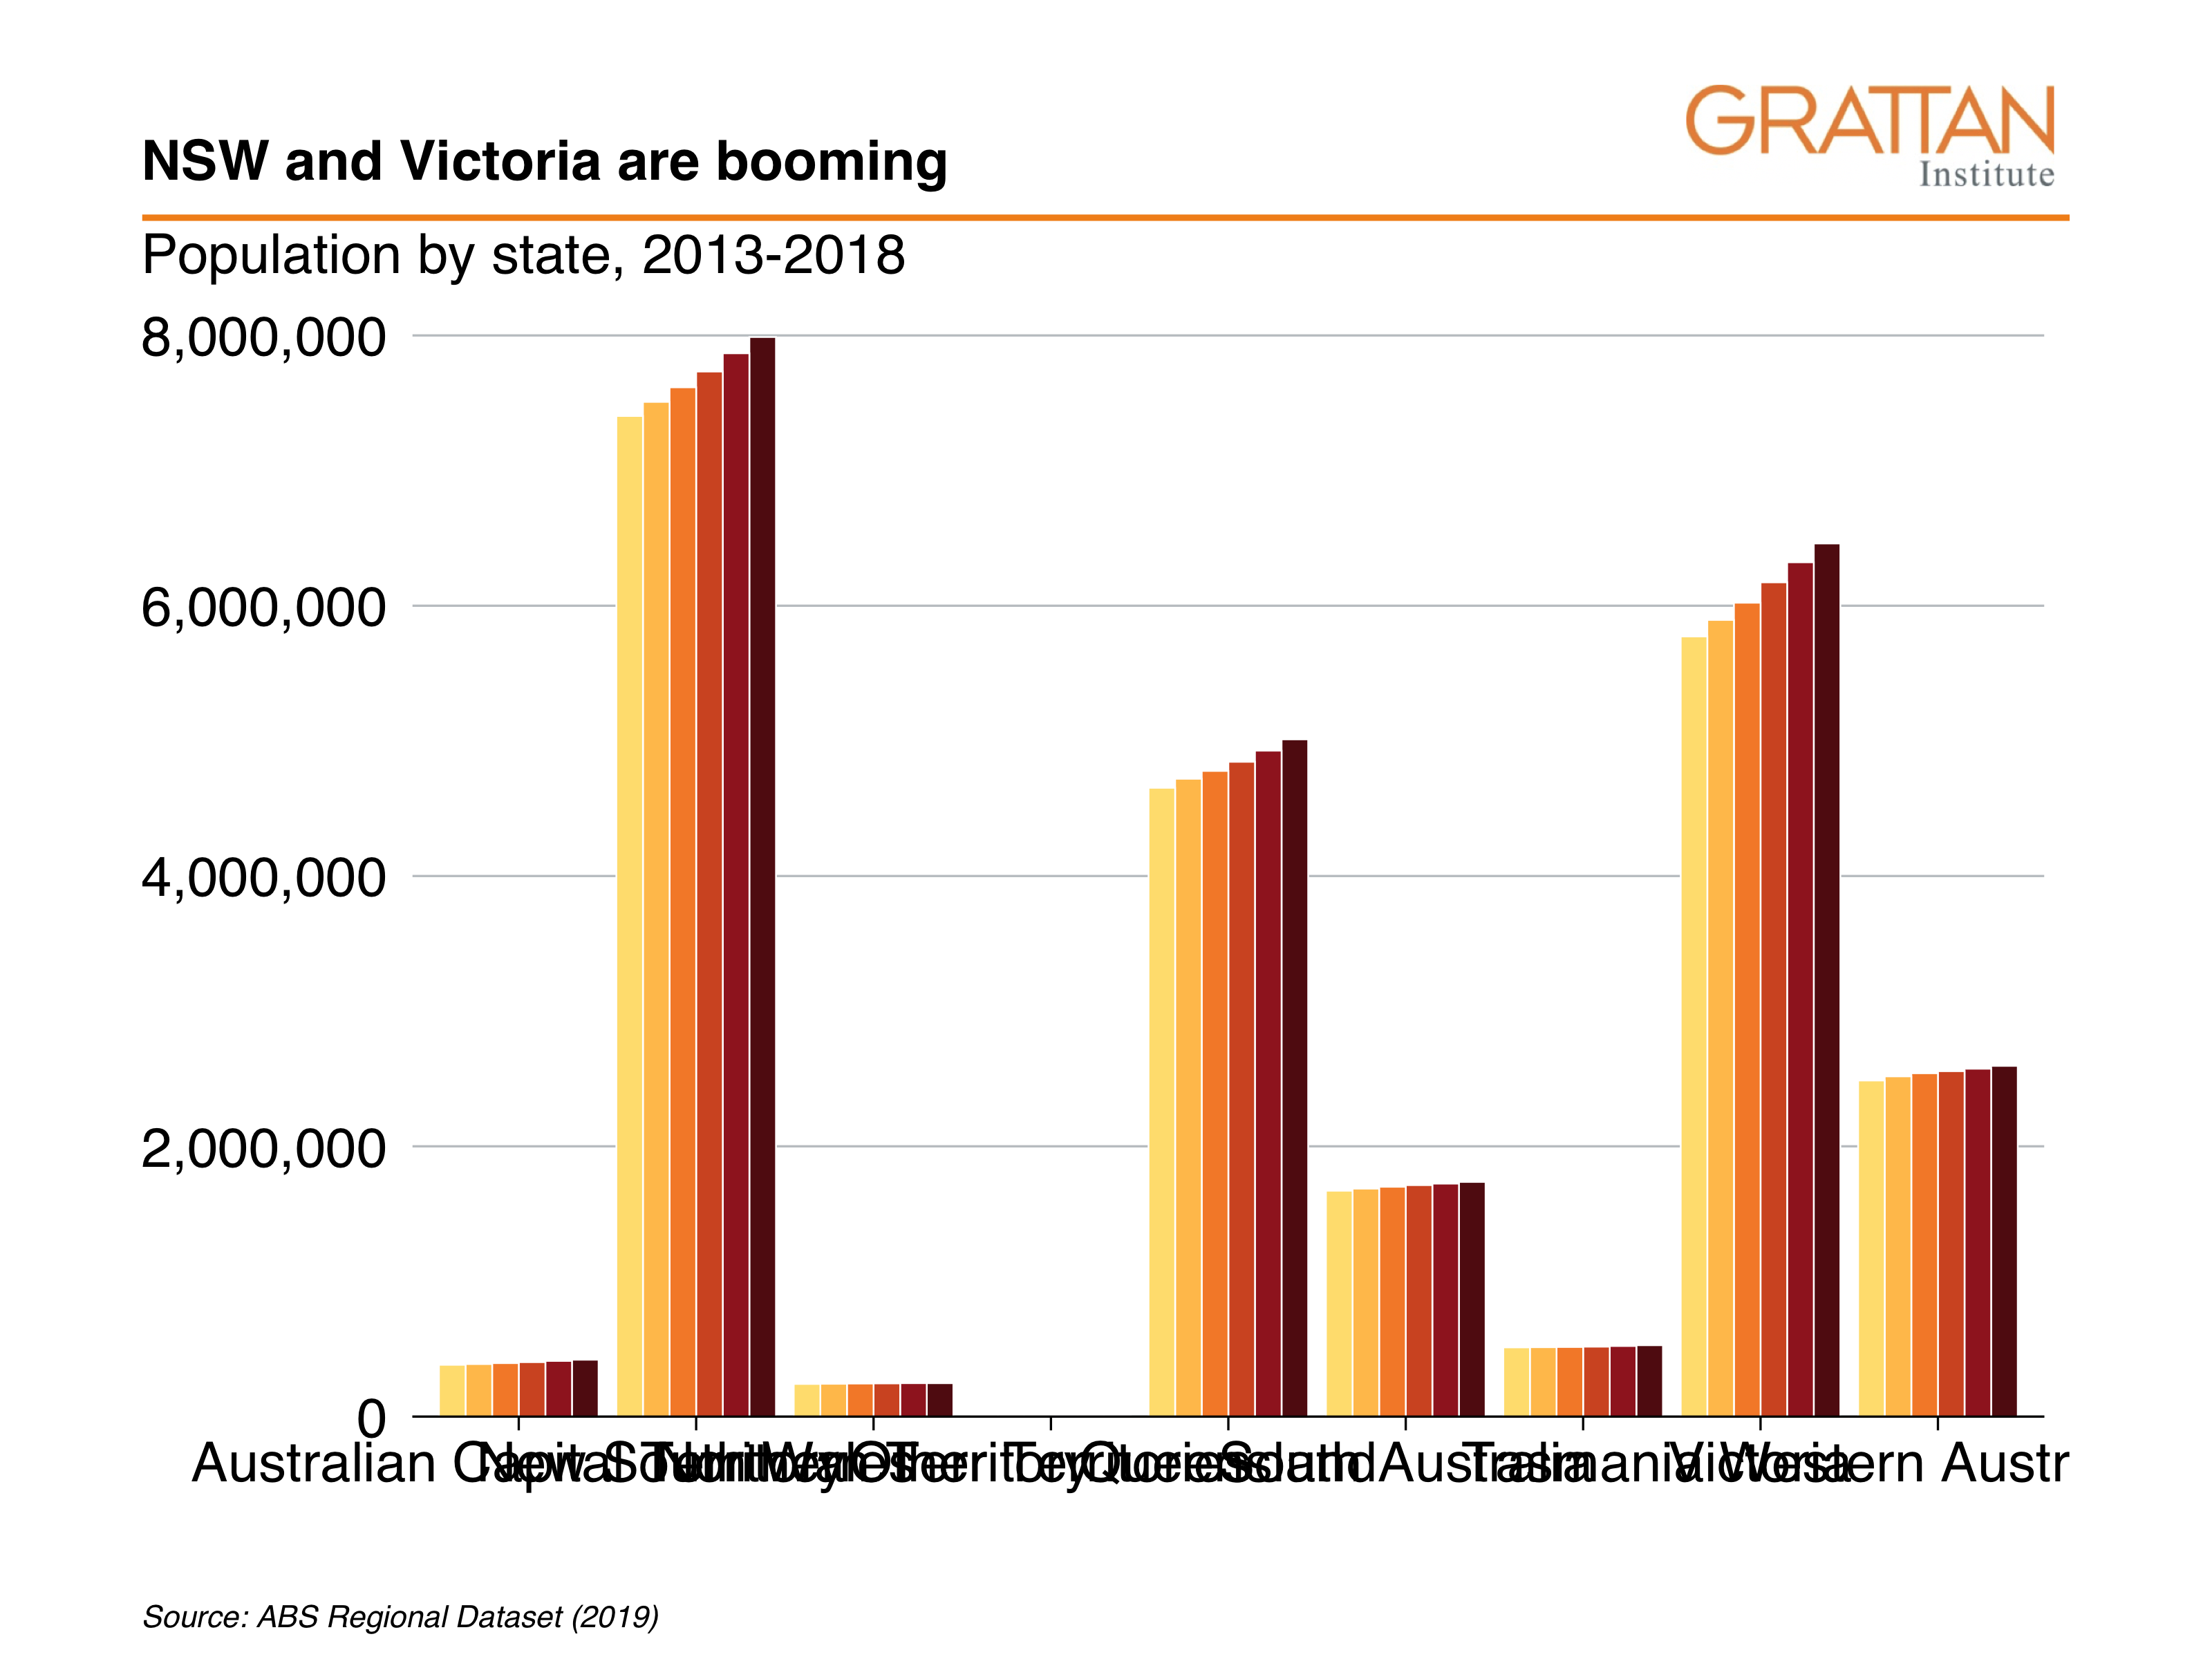
\includegraphics{atlas/population_chart_presentation.png}

Or, if you want to emphasise the point in a \emph{really tall} chart for a \textbf{blogpost}, you can use \texttt{type\ =\ "blog"} and adjust the \texttt{height} to be 50cm. Also note that because this is for the blog, you should save it as a \texttt{png} file:

\begin{Shaded}
\begin{Highlighting}[]
\KeywordTok{grattan_save}\NormalTok{(}\StringTok{"atlas/population_chart_blog.png"}\NormalTok{, pop_chart, }
             \DataTypeTok{type =} \StringTok{"blog"}\NormalTok{, }\DataTypeTok{height =} \DecValTok{50}\NormalTok{)}
\end{Highlighting}
\end{Shaded}

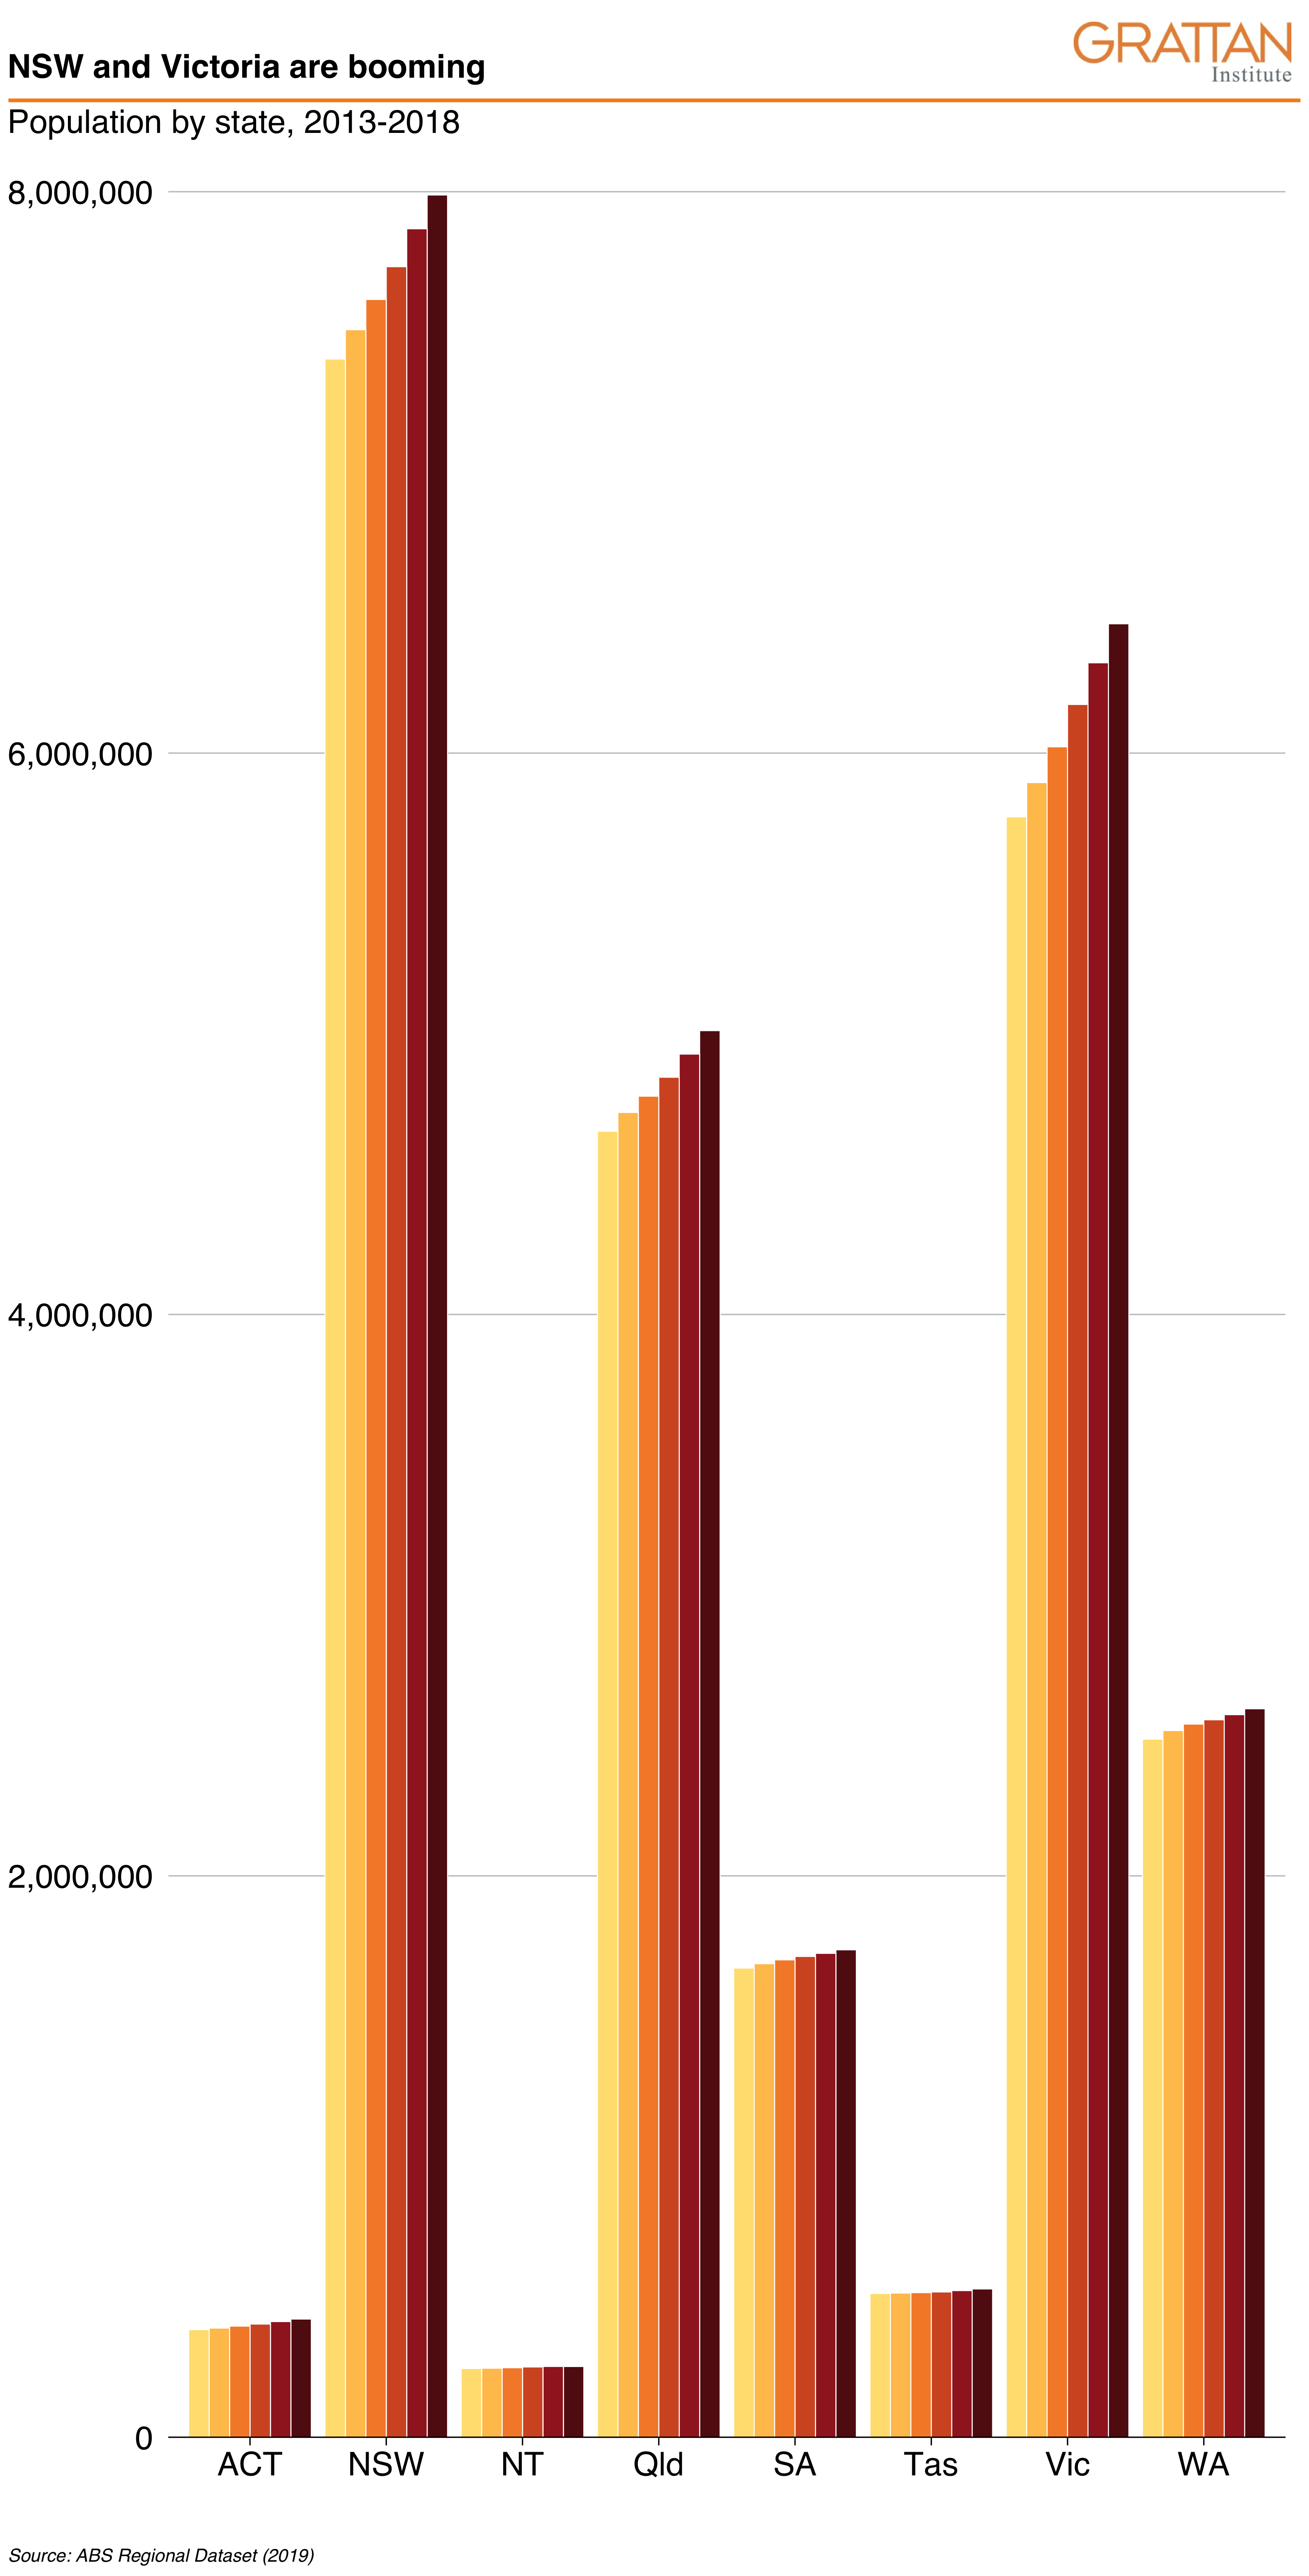
\includegraphics{atlas/population_chart_blog.png}

And that's it! The following sections will go into more detail about different chart types in R, but you'll mostly use the same basic \texttt{grattantheme} formatting you've used here.

\hypertarget{chart-cookbook}{%
\section{Chart cookbook}\label{chart-cookbook}}

This section takes you through a few often-used chart types.

\hypertarget{bar-charts}{%
\subsection{Bar charts}\label{bar-charts}}

Bar charts are made with \texttt{geom\_bar} or \texttt{geom\_col}. Creating a bar chart will look something like this:

\begin{Shaded}
\begin{Highlighting}[]
\KeywordTok{ggplot}\NormalTok{(}\DataTypeTok{data =} \OperatorTok{<}\NormalTok{data}\OperatorTok{>}\NormalTok{) }\OperatorTok{+}\StringTok{ }
\StringTok{  }\KeywordTok{geom_bar}\NormalTok{(}\KeywordTok{aes}\NormalTok{(}\DataTypeTok{x =} \OperatorTok{<}\NormalTok{xvar}\OperatorTok{>}\NormalTok{, }\DataTypeTok{y =} \OperatorTok{<}\NormalTok{yvar}\OperatorTok{>}\NormalTok{),}
     \DataTypeTok{stat =} \OperatorTok{<}\NormalTok{STAT}\OperatorTok{>}\NormalTok{, }
     \DataTypeTok{position =} \OperatorTok{<}\NormalTok{POSITION}\OperatorTok{>}
\StringTok{  }\NormalTok{)}
\end{Highlighting}
\end{Shaded}

It has two key arguments: \texttt{stat} and \texttt{position}.

First, \texttt{stat} defines what kind of \emph{operation} the function will do on the dataset before plotting. Some options are:

\begin{itemize}
\tightlist
\item
  \texttt{"count"}, the default: count the number of observations in a particular group, and plot that number. This is useful when you're using microdata. When this is the case, there is no need for a \texttt{y} aesthetic.
\item
  \texttt{"sum"}: sum the values of the \texttt{y} aesthetic.
\item
  \texttt{"identity"}: directly report the values of the \texttt{y} aesthetic. This is how Powerpoint and Excel charts work.
\end{itemize}

You can use \texttt{geom\_col} instead, as a shortcut for \texttt{geom\_bar(stat\ =\ "identity)}.

Second, \texttt{position}, dictates how multiple bars occupying the same x-axis position will positioned. The options are:

\begin{itemize}
\tightlist
\item
  \texttt{"stack"}, the default: bars in the same group are stacked atop one another.
\item
  \texttt{"dodge"}: bars in the same group are positioned next to one another.
\item
  \texttt{"fill"}: bars in the same group are stacked and all fill to 100 per cent.
\end{itemize}

\begin{Shaded}
\begin{Highlighting}[]
\NormalTok{population_table }\OperatorTok\StringTok{ }
\StringTok{        }\KeywordTok{ggplot}\NormalTok{(}\KeywordTok{aes}\NormalTok{(}\DataTypeTok{x =}\NormalTok{ state,}
                   \DataTypeTok{y =}\NormalTok{ pop,}
                   \DataTypeTok{fill =}\NormalTok{ year)) }\OperatorTok{+}
\StringTok{        }\KeywordTok{geom_bar}\NormalTok{(}\DataTypeTok{stat =} \StringTok{"identity"}\NormalTok{,}
                 \DataTypeTok{position =} \StringTok{"dodge"}\NormalTok{) }\OperatorTok{+}
\StringTok{        }\KeywordTok{theme_grattan}\NormalTok{() }\OperatorTok{+}
\StringTok{        }\KeywordTok{grattan_y_continuous}\NormalTok{(}\DataTypeTok{labels =}\NormalTok{ comma) }\OperatorTok{+}
\StringTok{        }\KeywordTok{grattan_fill_manual}\NormalTok{(}\DecValTok{6}\NormalTok{)}
\end{Highlighting}
\end{Shaded}

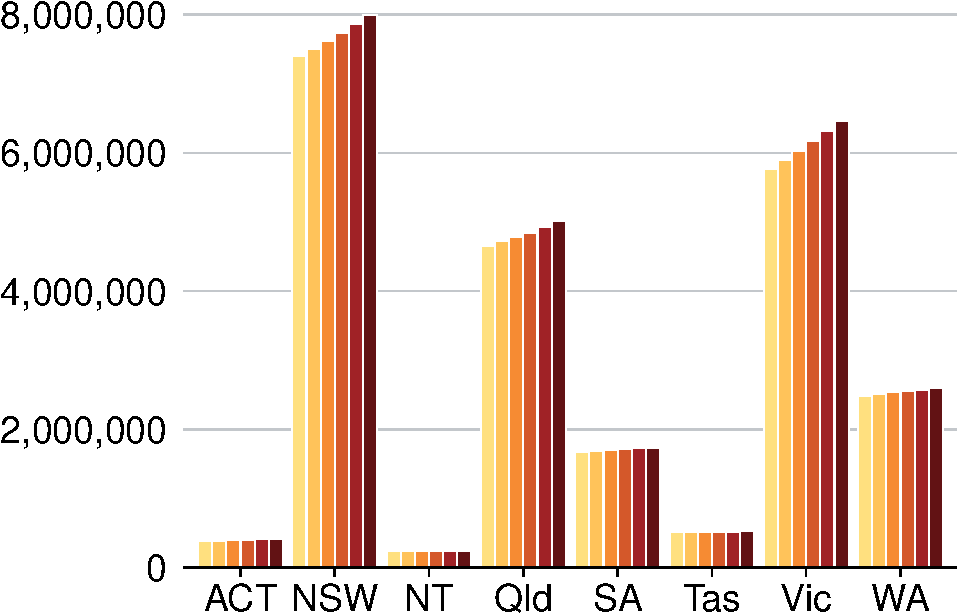
\includegraphics{Data_visualisation_files/figure-latex/bar2-1.pdf}

You can also \textbf{order} the groups in your chart by a variable. If you want to order states by population, use \texttt{reorder} inside \texttt{aes}:

\begin{Shaded}
\begin{Highlighting}[]
\NormalTok{population_table }\OperatorTok\StringTok{ }
\StringTok{        }\KeywordTok{ggplot}\NormalTok{(}\KeywordTok{aes}\NormalTok{(}\DataTypeTok{x =} \KeywordTok{reorder}\NormalTok{(state, }\OperatorTok{-}\NormalTok{pop), }\CommentTok{# reorder state by negative population}
                   \DataTypeTok{y =}\NormalTok{ pop,}
                   \DataTypeTok{fill =}\NormalTok{ year)) }\OperatorTok{+}
\StringTok{        }\KeywordTok{geom_bar}\NormalTok{(}\DataTypeTok{stat =} \StringTok{"identity"}\NormalTok{,}
                 \DataTypeTok{position =} \StringTok{"dodge"}\NormalTok{) }\OperatorTok{+}
\StringTok{        }\KeywordTok{theme_grattan}\NormalTok{() }\OperatorTok{+}
\StringTok{        }\KeywordTok{grattan_y_continuous}\NormalTok{(}\DataTypeTok{labels =}\NormalTok{ comma) }\OperatorTok{+}
\StringTok{        }\KeywordTok{grattan_fill_manual}\NormalTok{(}\DecValTok{6}\NormalTok{) }\OperatorTok{+}\StringTok{ }
\StringTok{        }\KeywordTok{labs}\NormalTok{(}\DataTypeTok{x =} \StringTok{""}\NormalTok{)}
\end{Highlighting}
\end{Shaded}

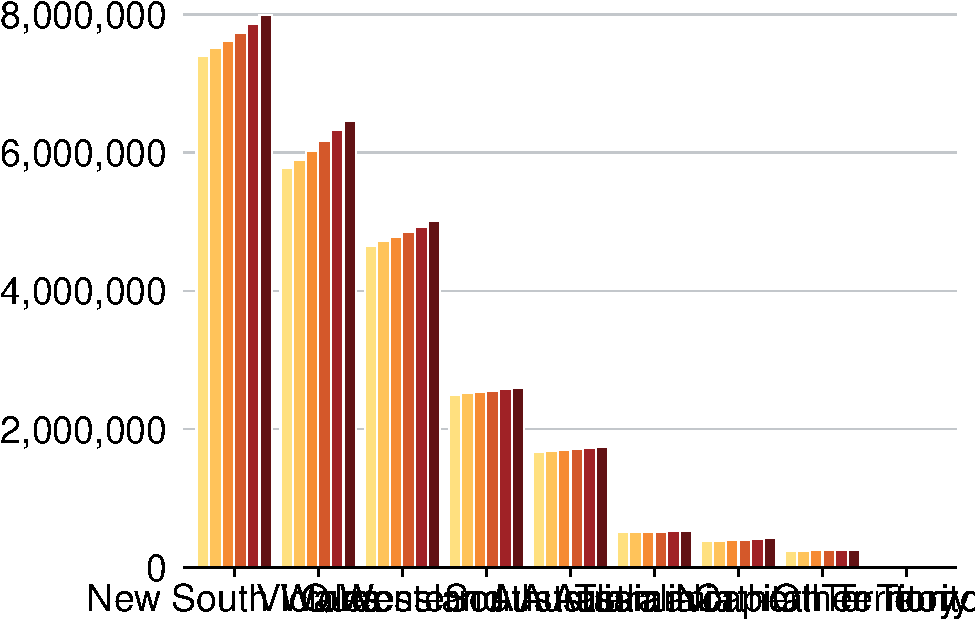
\includegraphics{Data_visualisation_files/figure-latex/bar3-1.pdf}

To flip the chart -- a useful move when you have long labels -- add \texttt{coord\_flipped} (ie `flip coordinates') and tell \texttt{theme\_grattan} that the plot is flipped using \texttt{flipped\ =\ TRUE}.

\begin{Shaded}
\begin{Highlighting}[]
\NormalTok{population_table }\OperatorTok\StringTok{ }
\StringTok{        }\KeywordTok{ggplot}\NormalTok{(}\KeywordTok{aes}\NormalTok{(}\DataTypeTok{x =} \KeywordTok{reorder}\NormalTok{(state, }\OperatorTok{-}\NormalTok{pop), }
                   \DataTypeTok{y =}\NormalTok{ pop,}
                   \DataTypeTok{fill =}\NormalTok{ year)) }\OperatorTok{+}
\StringTok{        }\KeywordTok{geom_bar}\NormalTok{(}\DataTypeTok{stat =} \StringTok{"identity"}\NormalTok{,}
                 \DataTypeTok{position =} \StringTok{"dodge"}\NormalTok{) }\OperatorTok{+}
\StringTok{        }\KeywordTok{coord_flip}\NormalTok{() }\OperatorTok{+}\StringTok{  }\CommentTok{# flip the coordinates}
\StringTok{        }\KeywordTok{theme_grattan}\NormalTok{(}\DataTypeTok{flipped =} \OtherTok{TRUE}\NormalTok{) }\OperatorTok{+}\StringTok{  }\CommentTok{# tell theme_grattan}
\StringTok{        }\KeywordTok{grattan_y_continuous}\NormalTok{(}\DataTypeTok{labels =}\NormalTok{ comma) }\OperatorTok{+}
\StringTok{        }\KeywordTok{grattan_fill_manual}\NormalTok{(}\DecValTok{6}\NormalTok{) }\OperatorTok{+}\StringTok{ }
\StringTok{        }\KeywordTok{labs}\NormalTok{(}\DataTypeTok{x =} \StringTok{""}\NormalTok{)}
\end{Highlighting}
\end{Shaded}

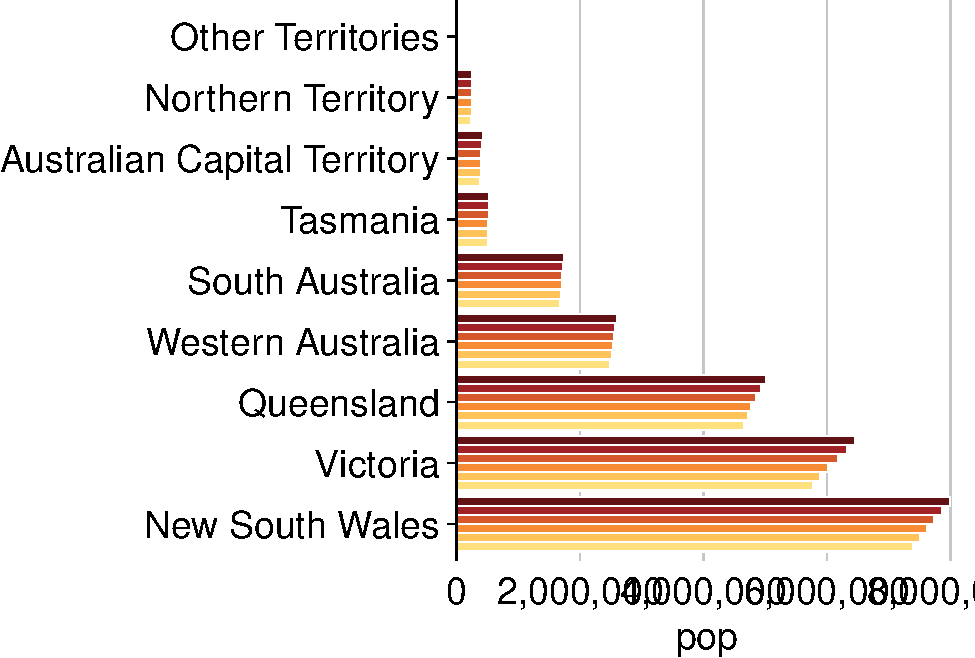
\includegraphics{Data_visualisation_files/figure-latex/bar4-1.pdf}

\hypertarget{line-charts}{%
\subsection{Line charts}\label{line-charts}}

A line chart has one key aesthetic: \texttt{group}. This tells \texttt{ggplot} how to connect individual lines.

\begin{Shaded}
\begin{Highlighting}[]
\NormalTok{population_table }\OperatorTok\StringTok{ }
\StringTok{        }\KeywordTok{ggplot}\NormalTok{(}\KeywordTok{aes}\NormalTok{(}\DataTypeTok{x =}\NormalTok{ year,}
                   \DataTypeTok{y =}\NormalTok{ pop,}
                   \DataTypeTok{colour =}\NormalTok{ state,}
                   \DataTypeTok{group =}\NormalTok{ state)) }\OperatorTok{+}
\StringTok{        }\KeywordTok{geom_line}\NormalTok{() }\OperatorTok{+}
\StringTok{        }\KeywordTok{theme_grattan}\NormalTok{() }\OperatorTok{+}
\StringTok{        }\KeywordTok{grattan_y_continuous}\NormalTok{(}\DataTypeTok{labels =}\NormalTok{ comma) }\OperatorTok{+}
\StringTok{        }\KeywordTok{grattan_colour_manual}\NormalTok{(}\DecValTok{9}\NormalTok{) }\OperatorTok{+}
\StringTok{        }\KeywordTok{labs}\NormalTok{(}\DataTypeTok{x =} \StringTok{""}\NormalTok{)}
\end{Highlighting}
\end{Shaded}

\begin{verbatim}
## Warning in grattantheme::grattan_pal(n = n, reverse = reverse): Using more
## than six colours is not recommended.
\end{verbatim}

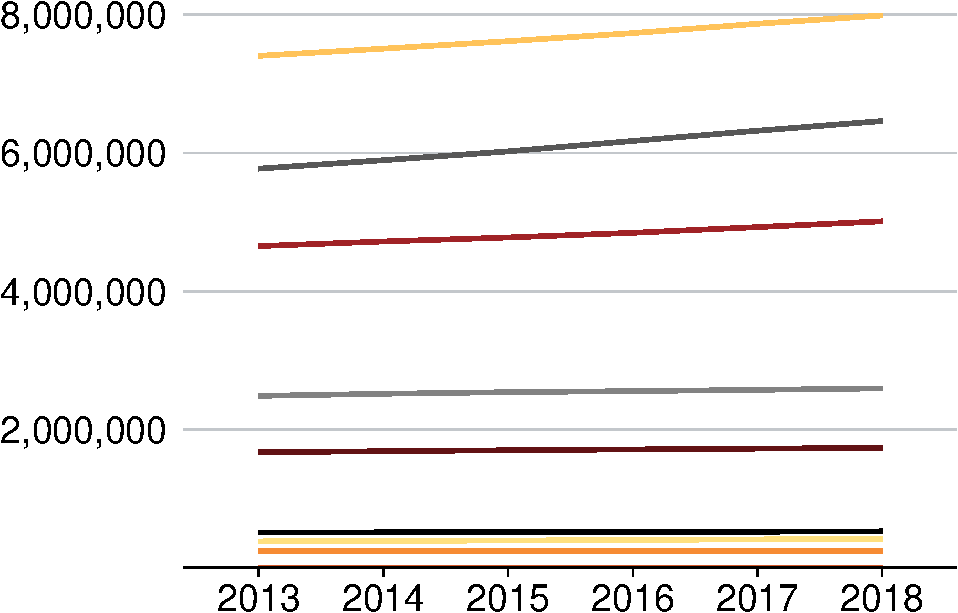
\includegraphics{Data_visualisation_files/figure-latex/line1-1.pdf}

You can also add dots for each year by layering \texttt{geom\_point} on top of \texttt{geom\_line}:

\begin{Shaded}
\begin{Highlighting}[]
\NormalTok{population_table }\OperatorTok\StringTok{ }
\StringTok{        }\KeywordTok{ggplot}\NormalTok{(}\KeywordTok{aes}\NormalTok{(}\DataTypeTok{x =}\NormalTok{ year,}
                   \DataTypeTok{y =}\NormalTok{ pop,}
                   \DataTypeTok{colour =}\NormalTok{ state,}
                   \DataTypeTok{group =}\NormalTok{ state)) }\OperatorTok{+}
\StringTok{        }\KeywordTok{geom_line}\NormalTok{() }\OperatorTok{+}
\StringTok{        }\KeywordTok{geom_point}\NormalTok{(}\DataTypeTok{size =} \DecValTok{2}\NormalTok{) }\OperatorTok{+}\StringTok{ }
\StringTok{        }\KeywordTok{theme_grattan}\NormalTok{() }\OperatorTok{+}
\StringTok{        }\KeywordTok{grattan_y_continuous}\NormalTok{(}\DataTypeTok{labels =}\NormalTok{ comma) }\OperatorTok{+}
\StringTok{        }\KeywordTok{grattan_colour_manual}\NormalTok{(}\DecValTok{9}\NormalTok{) }\OperatorTok{+}\StringTok{ }
\StringTok{        }\KeywordTok{labs}\NormalTok{(}\DataTypeTok{x =} \StringTok{""}\NormalTok{)}
\end{Highlighting}
\end{Shaded}

\begin{verbatim}
## Warning in grattantheme::grattan_pal(n = n, reverse = reverse): Using more
## than six colours is not recommended.
\end{verbatim}

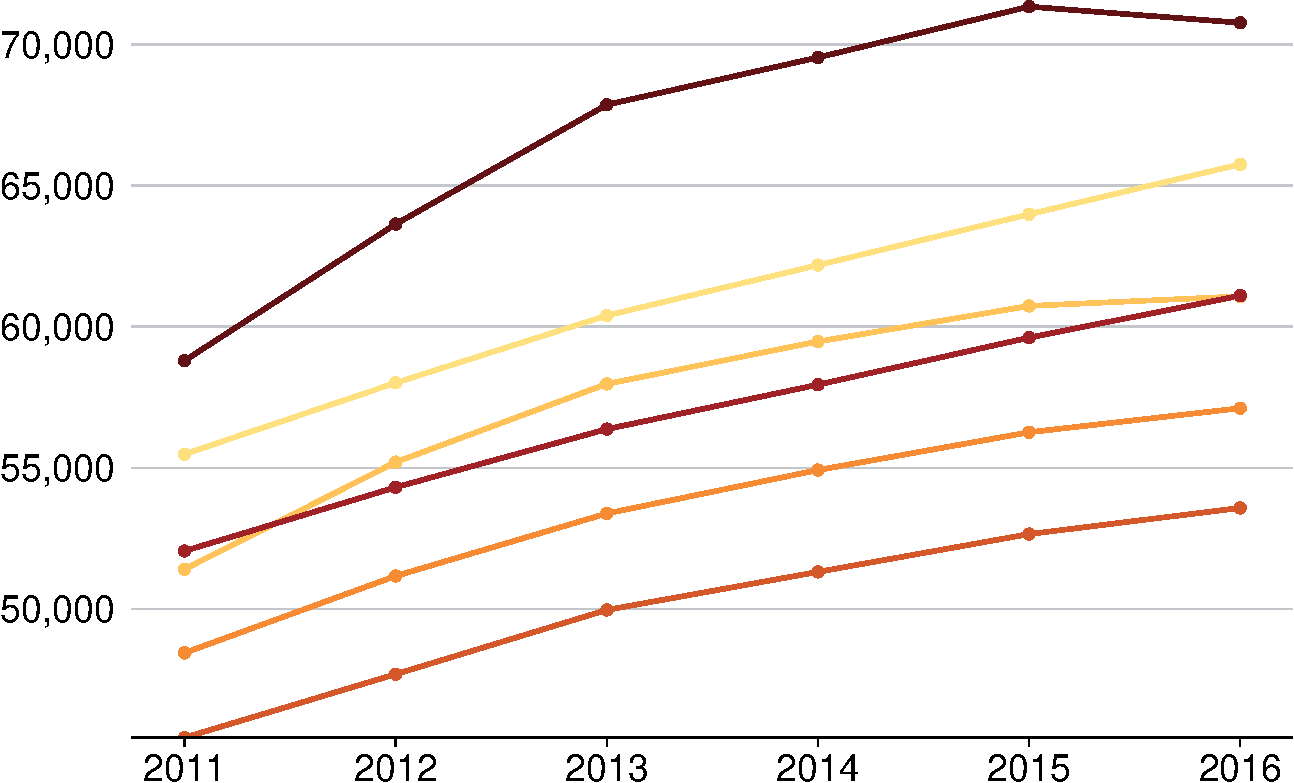
\includegraphics{Data_visualisation_files/figure-latex/line2-1.pdf}

If you wanted to show each state individually, you could \textbf{facet} your chart so that a separate plot was produced for each state:

\begin{Shaded}
\begin{Highlighting}[]
\NormalTok{population_table }\OperatorTok\StringTok{ }
\StringTok{        }\KeywordTok{filter}\NormalTok{(state }\OperatorTok{!=}\StringTok{ "ACT"}\NormalTok{,}
\NormalTok{               state }\OperatorTok{!=}\StringTok{ "NT"}\NormalTok{) }\OperatorTok\StringTok{ }
\StringTok{        }\KeywordTok{ggplot}\NormalTok{(}\KeywordTok{aes}\NormalTok{(}\DataTypeTok{x =}\NormalTok{ year,}
                   \DataTypeTok{y =}\NormalTok{ pop,}
                   \DataTypeTok{group =}\NormalTok{ state)) }\OperatorTok{+}
\StringTok{        }\KeywordTok{geom_line}\NormalTok{() }\OperatorTok{+}
\StringTok{        }\KeywordTok{geom_point}\NormalTok{(}\DataTypeTok{size =} \DecValTok{2}\NormalTok{) }\OperatorTok{+}\StringTok{ }
\StringTok{        }\KeywordTok{theme_grattan}\NormalTok{() }\OperatorTok{+}
\StringTok{        }\KeywordTok{grattan_y_continuous}\NormalTok{() }\OperatorTok{+}
\StringTok{        }\KeywordTok{facet_wrap}\NormalTok{(state }\OperatorTok{~}\StringTok{ }\NormalTok{.) }\OperatorTok{+}\StringTok{ }
\StringTok{        }\KeywordTok{labs}\NormalTok{(}\DataTypeTok{x =} \StringTok{""}\NormalTok{)}
\end{Highlighting}
\end{Shaded}

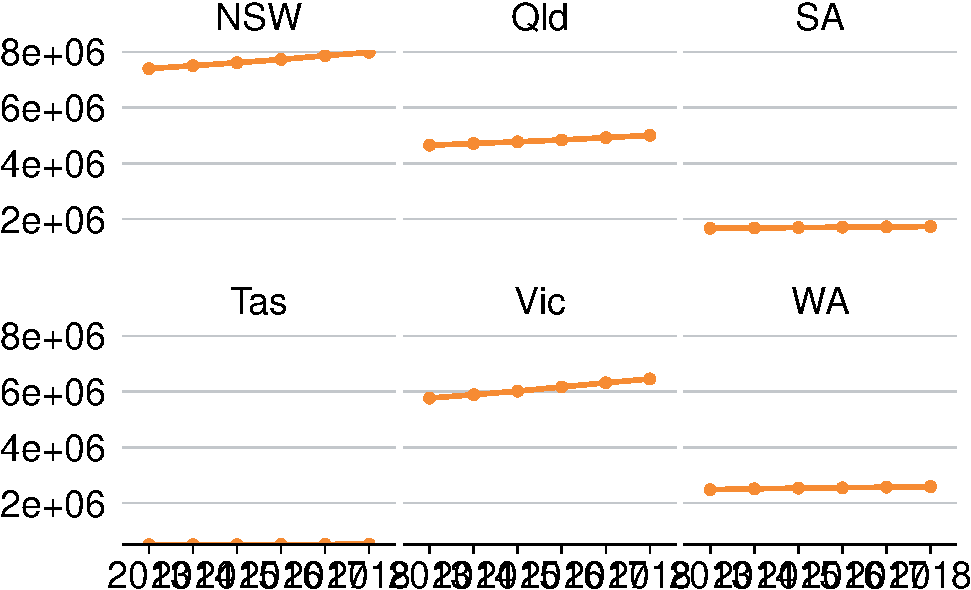
\includegraphics{Data_visualisation_files/figure-latex/line3-1.pdf}

To tidy this up, we can:

\begin{enumerate}
\def\labelenumi{\arabic{enumi}.}
\tightlist
\item
  shorten the years to be ``13'', ``14'', etc instead of ``2013'', ``2014'', etc (via the \texttt{x} aesthetic)
\item
  shorten the y-axis labels to ``millions'' (via the \texttt{y} aesthetic)
\item
  add a black horizontal line at the bottom of each facet
\item
  give the facets a bit of room by adjusting \texttt{panel.spacing}
\item
  define our own x-axis label breaks to just show \texttt{13}, \texttt{15} and \texttt{17}
\end{enumerate}

\begin{Shaded}
\begin{Highlighting}[]
\NormalTok{population_table }\OperatorTok\StringTok{ }
\StringTok{        }\KeywordTok{filter}\NormalTok{(state }\OperatorTok{!=}\StringTok{ "ACT"}\NormalTok{,}
\NormalTok{               state }\OperatorTok{!=}\StringTok{ "NT"}\NormalTok{) }\OperatorTok\StringTok{ }
\StringTok{        }\KeywordTok{ggplot}\NormalTok{(}\KeywordTok{aes}\NormalTok{(}\DataTypeTok{x =} \KeywordTok{substr}\NormalTok{(year, }\DecValTok{3}\NormalTok{, }\DecValTok{4}\NormalTok{), }\CommentTok{# 1: just take the last two characters}
                   \DataTypeTok{y =}\NormalTok{ pop }\OperatorTok{/}\StringTok{ }\FloatTok{1e6}\NormalTok{, }\CommentTok{# 2: divide population by one million}
                   \DataTypeTok{group =}\NormalTok{ state)) }\OperatorTok{+}
\StringTok{        }\KeywordTok{geom_line}\NormalTok{() }\OperatorTok{+}
\StringTok{        }\KeywordTok{geom_point}\NormalTok{(}\DataTypeTok{size =} \DecValTok{2}\NormalTok{) }\OperatorTok{+}\StringTok{ }
\StringTok{        }\KeywordTok{geom_hline}\NormalTok{(}\DataTypeTok{yintercept =} \DecValTok{0}\NormalTok{) }\OperatorTok{+}\StringTok{ }\CommentTok{# 3: add horizontal line at the bottom}
\StringTok{        }\KeywordTok{theme_grattan}\NormalTok{() }\OperatorTok{+}
\StringTok{        }\KeywordTok{theme}\NormalTok{(}\DataTypeTok{panel.spacing =} \KeywordTok{unit}\NormalTok{(}\DecValTok{10}\NormalTok{, }\StringTok{"mm"}\NormalTok{)) }\OperatorTok{+}\StringTok{ }\CommentTok{# 4: add panel spacing}
\StringTok{        }\KeywordTok{grattan_y_continuous}\NormalTok{(}\DataTypeTok{labels =}\NormalTok{ comma) }\OperatorTok{+}
\StringTok{        }\KeywordTok{scale_x_discrete}\NormalTok{(}\DataTypeTok{breaks =} \KeywordTok{c}\NormalTok{(}\StringTok{"13"}\NormalTok{, }\StringTok{"15"}\NormalTok{, }\StringTok{"17"}\NormalTok{)) }\OperatorTok{+}\StringTok{ }\CommentTok{# 5: define our own label breaks}
\StringTok{        }\KeywordTok{facet_wrap}\NormalTok{(state }\OperatorTok{~}\StringTok{ }\NormalTok{.) }\OperatorTok{+}\StringTok{ }
\StringTok{        }\KeywordTok{labs}\NormalTok{(}\DataTypeTok{x =} \StringTok{""}\NormalTok{)}
\end{Highlighting}
\end{Shaded}

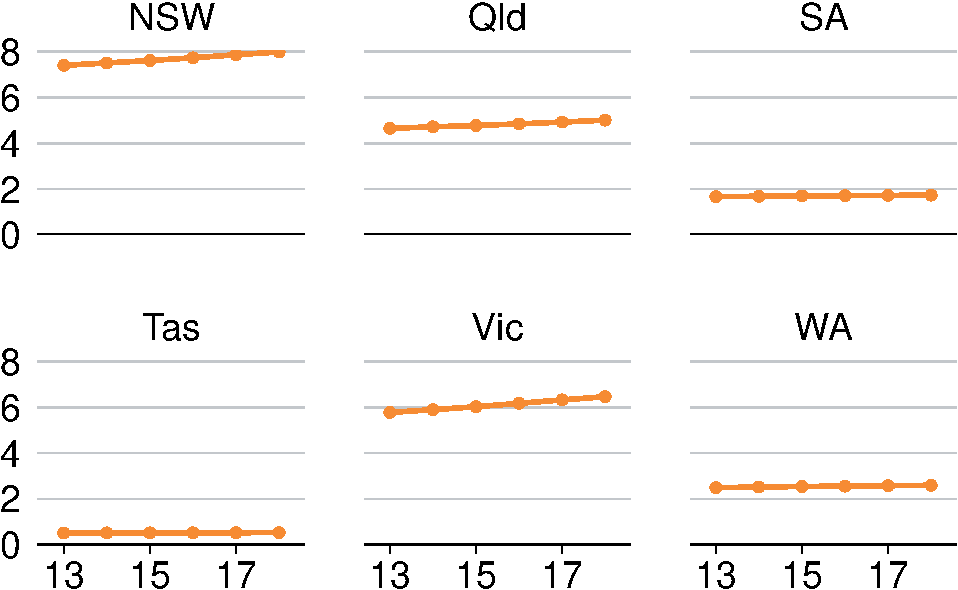
\includegraphics{Data_visualisation_files/figure-latex/line4-1.pdf}

\hypertarget{scatter-plots}{%
\subsection{Scatter plots}\label{scatter-plots}}

Scatter plots require \texttt{x} and \texttt{y} aesthetics. These can then be coloured and facetted.

First, create a dataset that we'll use for scatter plots. Take the \texttt{population\_table} dataset and transform it to have one variable for population in 2013, and another for population in 2018:

\begin{Shaded}
\begin{Highlighting}[]
\NormalTok{population_diff <-}\StringTok{ }\KeywordTok{read_csv}\NormalTok{(}\StringTok{"data/population_sa4.csv"}\NormalTok{) }\OperatorTok\StringTok{ }
\StringTok{        }\KeywordTok{mutate}\NormalTok{(}\DataTypeTok{state_long =}\NormalTok{ state,}
               \DataTypeTok{state =}\NormalTok{ strayr}\OperatorTok{::}\KeywordTok{strayr}\NormalTok{(state_long),}
               \DataTypeTok{pop =} \KeywordTok{as.numeric}\NormalTok{(value),}
               \DataTypeTok{year =} \KeywordTok{as.factor}\NormalTok{(glue}\OperatorTok{::}\KeywordTok{glue}\NormalTok{(}\StringTok{"y\{year\}"}\NormalTok{))) }\OperatorTok\StringTok{ }
\StringTok{        }\KeywordTok{filter}\NormalTok{(year }\OperatorTok\StringTok{ }\KeywordTok{c}\NormalTok{(}\StringTok{"y2013"}\NormalTok{, }\StringTok{"y2018"}\NormalTok{),}
\NormalTok{               data_item }\OperatorTok{==}\StringTok{ "Persons - Total (no.)"}\NormalTok{,}
\NormalTok{               sa4_name }\OperatorTok{!=}\StringTok{ "Other Territories"}\NormalTok{) }\OperatorTok\StringTok{ }
\StringTok{        }\KeywordTok{group_by}\NormalTok{(year, state, sa4_name) }\OperatorTok\StringTok{ }
\StringTok{        }\KeywordTok{summarise}\NormalTok{(}\DataTypeTok{pop =} \KeywordTok{sum}\NormalTok{(pop)) }\OperatorTok\StringTok{ }
\StringTok{        }\KeywordTok{spread}\NormalTok{(year, pop) }\OperatorTok\StringTok{ }
\StringTok{        }\KeywordTok{mutate}\NormalTok{(}\DataTypeTok{pop_change =} \DecValTok{100} \OperatorTok{*}\StringTok{ }\NormalTok{(y2018 }\OperatorTok{/}\StringTok{ }\NormalTok{y2013 }\OperatorTok{-}\StringTok{ }\DecValTok{1}\NormalTok{))}
\end{Highlighting}
\end{Shaded}

\begin{Shaded}
\begin{Highlighting}[]
\NormalTok{population_diff }\OperatorTok\StringTok{ }
\StringTok{        }\KeywordTok{ggplot}\NormalTok{(}\KeywordTok{aes}\NormalTok{(}\DataTypeTok{x =}\NormalTok{ y2013}\OperatorTok{/}\DecValTok{1000}\NormalTok{,}
                   \DataTypeTok{y =}\NormalTok{ pop_change)) }\OperatorTok{+}
\StringTok{        }\KeywordTok{geom_point}\NormalTok{(}\DataTypeTok{size =} \DecValTok{4}\NormalTok{) }\OperatorTok{+}\StringTok{ }
\StringTok{        }\KeywordTok{theme_grattan}\NormalTok{() }\OperatorTok{+}
\StringTok{        }\KeywordTok{theme}\NormalTok{(}\DataTypeTok{axis.title.y =} \KeywordTok{element_text}\NormalTok{(}\DataTypeTok{angle =} \DecValTok{90}\NormalTok{)) }\OperatorTok{+}
\StringTok{        }\KeywordTok{grattan_y_continuous}\NormalTok{() }\OperatorTok{+}\StringTok{ }
\StringTok{        }\KeywordTok{labs}\NormalTok{(}\DataTypeTok{y =} \StringTok{"Population increase to 2018, per cent"}\NormalTok{,}
             \DataTypeTok{x =} \StringTok{"Population in 2013, thousands"}\NormalTok{)}
\end{Highlighting}
\end{Shaded}

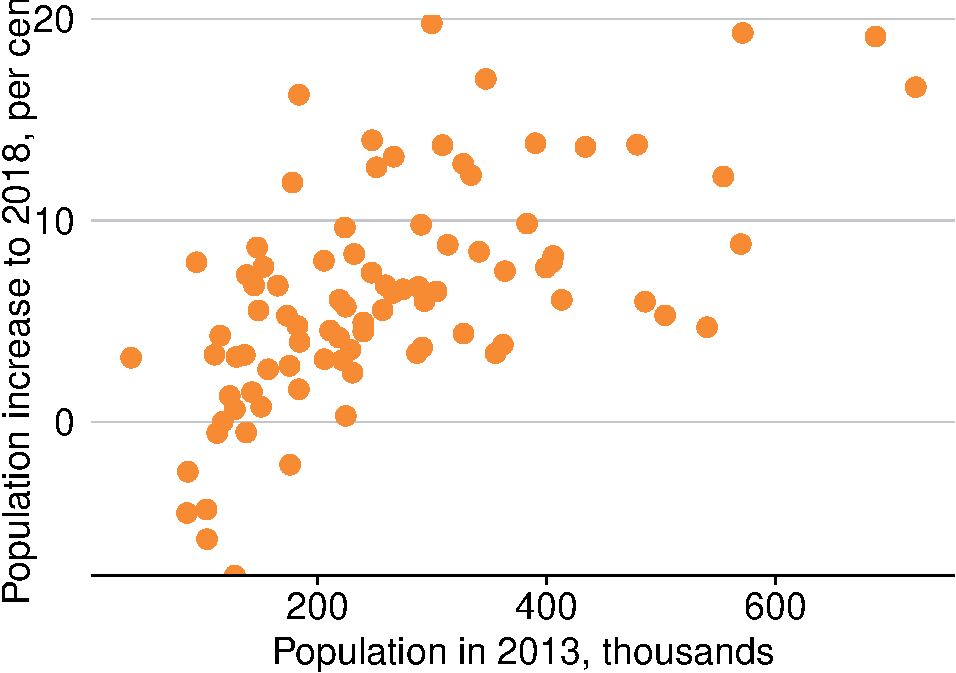
\includegraphics{Data_visualisation_files/figure-latex/scatter1-1.pdf}

It looks like the areas with the largest population grew the most between 2013 and 2018. To explore the relationship further, you can add a line-of-best-fit with \texttt{geom\_smooth}:

\begin{Shaded}
\begin{Highlighting}[]
\NormalTok{population_diff }\OperatorTok\StringTok{ }
\StringTok{        }\KeywordTok{ggplot}\NormalTok{(}\KeywordTok{aes}\NormalTok{(}\DataTypeTok{x =}\NormalTok{ y2013}\OperatorTok{/}\DecValTok{1000}\NormalTok{,  }\CommentTok{# display the x-axis as thousands}
                   \DataTypeTok{y =}\NormalTok{ pop_change)) }\OperatorTok{+}
\StringTok{        }\KeywordTok{geom_point}\NormalTok{(}\DataTypeTok{size =} \DecValTok{4}\NormalTok{) }\OperatorTok{+}\StringTok{ }
\StringTok{        }\KeywordTok{geom_smooth}\NormalTok{() }\OperatorTok{+}\StringTok{ }
\StringTok{        }\KeywordTok{geom_hline}\NormalTok{(}\DataTypeTok{yintercept =} \DecValTok{0}\NormalTok{) }\OperatorTok{+}
\StringTok{        }\KeywordTok{theme_grattan}\NormalTok{() }\OperatorTok{+}
\StringTok{        }\KeywordTok{theme}\NormalTok{(}\DataTypeTok{axis.title.y =} \KeywordTok{element_text}\NormalTok{(}\DataTypeTok{angle =} \DecValTok{90}\NormalTok{)) }\OperatorTok{+}
\StringTok{        }\KeywordTok{grattan_y_continuous}\NormalTok{() }\OperatorTok{+}\StringTok{ }
\StringTok{        }\KeywordTok{labs}\NormalTok{(}\DataTypeTok{y =} \StringTok{"Population increase to 2018, per cent"}\NormalTok{,}
             \DataTypeTok{x =} \StringTok{"Population in 2013, thousands"}\NormalTok{)}
\end{Highlighting}
\end{Shaded}

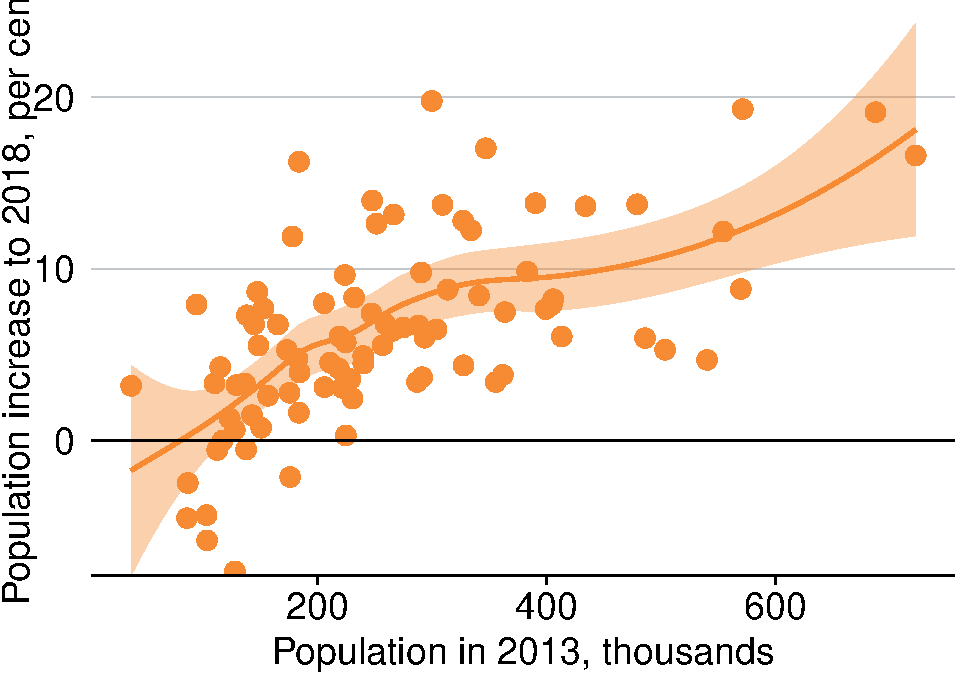
\includegraphics{Data_visualisation_files/figure-latex/scatter2-1.pdf}

You could colour-code positive and negative changes from within the \texttt{geom\_point} aesthetic. Making a change there won't pass through to the \texttt{geom\_smooth} aesthetic, so your line-of-best-fit will apply to all data points.

\begin{Shaded}
\begin{Highlighting}[]
\NormalTok{population_diff }\OperatorTok\StringTok{ }
\StringTok{        }\KeywordTok{ggplot}\NormalTok{(}\KeywordTok{aes}\NormalTok{(}\DataTypeTok{x =}\NormalTok{ y2013}\OperatorTok{/}\DecValTok{1000}\NormalTok{,  }\CommentTok{# display the x-axis as thousands}
                   \DataTypeTok{y =}\NormalTok{ pop_change)) }\OperatorTok{+}
\StringTok{        }\KeywordTok{geom_point}\NormalTok{(}\KeywordTok{aes}\NormalTok{(}\DataTypeTok{colour =}\NormalTok{ pop_change }\OperatorTok{<}\StringTok{ }\DecValTok{0}\NormalTok{),}
                   \DataTypeTok{size =} \DecValTok{4}\NormalTok{) }\OperatorTok{+}\StringTok{ }
\StringTok{        }\KeywordTok{geom_smooth}\NormalTok{() }\OperatorTok{+}\StringTok{ }
\StringTok{        }\KeywordTok{geom_hline}\NormalTok{(}\DataTypeTok{yintercept =} \DecValTok{0}\NormalTok{) }\OperatorTok{+}
\StringTok{        }\KeywordTok{theme_grattan}\NormalTok{() }\OperatorTok{+}
\StringTok{        }\KeywordTok{theme}\NormalTok{(}\DataTypeTok{axis.title.y =} \KeywordTok{element_text}\NormalTok{(}\DataTypeTok{angle =} \DecValTok{90}\NormalTok{)) }\OperatorTok{+}
\StringTok{        }\KeywordTok{grattan_y_continuous}\NormalTok{() }\OperatorTok{+}\StringTok{ }
\StringTok{        }\KeywordTok{grattan_colour_manual}\NormalTok{(}\DecValTok{2}\NormalTok{) }\OperatorTok{+}
\StringTok{        }\KeywordTok{labs}\NormalTok{(}\DataTypeTok{y =} \StringTok{"Population increase to 2018, per cent"}\NormalTok{,}
             \DataTypeTok{x =} \StringTok{"Population in 2013, thousands"}\NormalTok{)}
\end{Highlighting}
\end{Shaded}

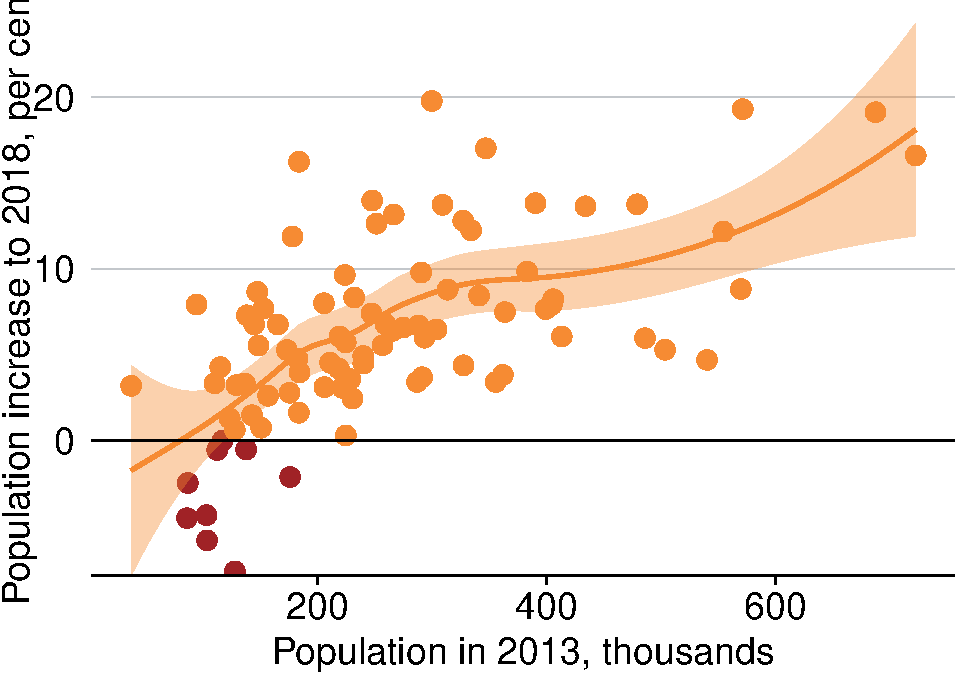
\includegraphics{Data_visualisation_files/figure-latex/scatter3-1.pdf}

Like the charts above, you could facet this by state to see if there were any interesting patterns. We'll filter out ACT and NT because they only have one and two data points (SA4s) in them, respectively.

\begin{Shaded}
\begin{Highlighting}[]
\NormalTok{population_diff }\OperatorTok\StringTok{ }
\StringTok{        }\KeywordTok{filter}\NormalTok{(state }\OperatorTok{!=}\StringTok{ "ACT"}\NormalTok{,}
\NormalTok{               state }\OperatorTok{!=}\StringTok{ "NT"}\NormalTok{) }\OperatorTok\StringTok{ }
\StringTok{        }\KeywordTok{ggplot}\NormalTok{(}\KeywordTok{aes}\NormalTok{(}\DataTypeTok{x =}\NormalTok{ y2013}\OperatorTok{/}\DecValTok{1000}\NormalTok{,  }\CommentTok{# display the x-axis as thousands}
                   \DataTypeTok{y =}\NormalTok{ pop_change)) }\OperatorTok{+}
\StringTok{        }\KeywordTok{geom_point}\NormalTok{(}\KeywordTok{aes}\NormalTok{(}\DataTypeTok{colour =}\NormalTok{ pop_change }\OperatorTok{<}\StringTok{ }\DecValTok{0}\NormalTok{),}
                   \DataTypeTok{size =} \DecValTok{2}\NormalTok{) }\OperatorTok{+}
\StringTok{        }\KeywordTok{geom_smooth}\NormalTok{() }\OperatorTok{+}\StringTok{ }
\StringTok{        }\KeywordTok{geom_hline}\NormalTok{(}\DataTypeTok{yintercept =} \DecValTok{0}\NormalTok{) }\OperatorTok{+}
\StringTok{        }\KeywordTok{theme_grattan}\NormalTok{() }\OperatorTok{+}
\StringTok{        }\KeywordTok{theme}\NormalTok{(}\DataTypeTok{axis.title.y =} \KeywordTok{element_text}\NormalTok{(}\DataTypeTok{angle =} \DecValTok{90}\NormalTok{)) }\OperatorTok{+}
\StringTok{        }\KeywordTok{grattan_y_continuous}\NormalTok{() }\OperatorTok{+}\StringTok{ }
\StringTok{        }\KeywordTok{grattan_colour_manual}\NormalTok{(}\DecValTok{2}\NormalTok{) }\OperatorTok{+}
\StringTok{        }\KeywordTok{labs}\NormalTok{(}\DataTypeTok{y =} \StringTok{"Population increase to 2018, per cent"}\NormalTok{,}
             \DataTypeTok{x =} \StringTok{"Population in 2013, thousands"}\NormalTok{) }\OperatorTok{+}
\StringTok{        }\KeywordTok{facet_wrap}\NormalTok{(state }\OperatorTok{~}\StringTok{ }\NormalTok{.)}
\end{Highlighting}
\end{Shaded}

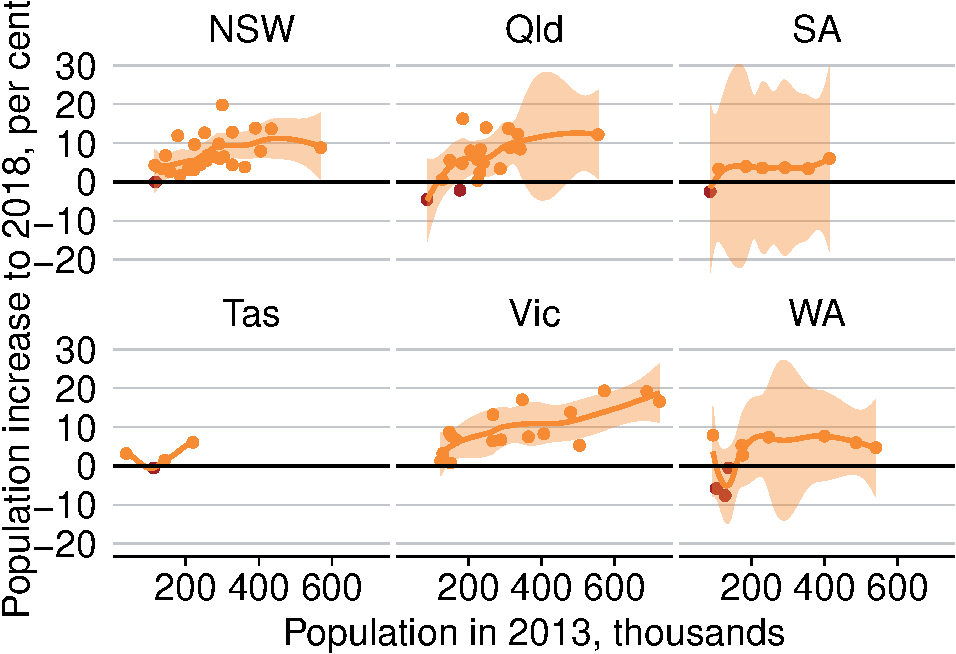
\includegraphics{Data_visualisation_files/figure-latex/scatter4-1.pdf}

\hypertarget{distributions}{%
\subsection{Distributions}\label{distributions}}

\texttt{geom\_histogram}
\texttt{geom\_density}

\texttt{ggridges::}

\hypertarget{maps}{%
\subsection{Maps}\label{maps}}

\hypertarget{sf-objects}{%
\subsubsection{\texorpdfstring{\texttt{sf} objects}{sf objects}}\label{sf-objects}}

{[}what is{]}

\hypertarget{using-absmapsdata}{%
\subsubsection{\texorpdfstring{Using \texttt{absmapsdata}}{Using absmapsdata}}\label{using-absmapsdata}}

The \texttt{absmapsdata} contains compressed, and tidied \texttt{sf} objects containing geometric information about ABS data structures. The included objects are:

\begin{itemize}
\tightlist
\item
  Statistical Area 1 2011: \texttt{sa12011}
\item
  Statistical Area 1 2016: \texttt{sa12016}
\item
  Statistical Area 2 2011: \texttt{sa22011}
\item
  Statistical Area 2 2016: \texttt{sa22016}
\item
  Statistical Area 3 2011: \texttt{sa32011}
\item
  Statistical Area 3 2016: \texttt{sa32016}
\item
  Statistical Area 4 2011: \texttt{sa42011}
\item
  Statistical Area 4 2016: \texttt{sa42016}
\item
  Greater Capital Cities 2011: \texttt{gcc2011}
\item
  Greater Capital Cities 2016: \texttt{gcc2016}
\item
  Remoteness Areas 2011: \texttt{ra2011}
\item
  Remoteness Areas 2016: \texttt{ra2016}
\item
  State 2011: \texttt{state2011}
\item
  State 2016: \texttt{state2016}
\item
  Commonwealth Electoral Divisions 2018: \texttt{ced2018}
\item
  State Electoral Divisions 2018:\texttt{sed2018}
\item
  Local Government Areas 2016: \texttt{lga2016}
\item
  Local Government Areas 2018: \texttt{lga2018}
\end{itemize}

You can install the package from Github. You will also need the \texttt{sf} package installed to handle the \texttt{sf} objects.

\begin{Shaded}
\begin{Highlighting}[]
\NormalTok{devtools}\OperatorTok{::}\KeywordTok{install_github}\NormalTok{(}\StringTok{"wfmackey/absmapsdata"}\NormalTok{)}
\KeywordTok{library}\NormalTok{(absmapsdata)}

\KeywordTok{install.packages}\NormalTok{(}\StringTok{"sf"}\NormalTok{)}
\KeywordTok{library}\NormalTok{(sf)}
\end{Highlighting}
\end{Shaded}

\hypertarget{making-choropleth-maps}{%
\subsubsection{Making choropleth maps}\label{making-choropleth-maps}}

Choropleth maps break an area into `bits', and colours each `bit' according to a variable.

SA4 is the largest non-state statistical area in the ABS ASGS standard.

You can join the \texttt{sf} objects from \texttt{absmapsdata} to your dataset using \texttt{left\_join}. The variable names might be different -- eg \texttt{sa4\_name} compared to \texttt{sa4\_name\_2016} -- so use the \texttt{by} function to match them.

\begin{Shaded}
\begin{Highlighting}[]
\NormalTok{map_data <-}\StringTok{ }\NormalTok{population_diff }\OperatorTok\StringTok{ }
\StringTok{        }\KeywordTok{left_join}\NormalTok{(sa42016, }\DataTypeTok{by =} \KeywordTok{c}\NormalTok{(}\StringTok{"sa4_name"}\NormalTok{ =}\StringTok{ "sa4_name_2016"}\NormalTok{))}

\KeywordTok{head}\NormalTok{(map_data }\OperatorTok\StringTok{ }
\StringTok{       }\KeywordTok{select}\NormalTok{(sa4_name, geometry))}
\end{Highlighting}
\end{Shaded}

\begin{verbatim}
## # A tibble: 6 x 3
## # Groups:   state [2]
##   state sa4_name                                                   geometry
##   <chr> <chr>                                            <MULTIPOLYGON [°]>
## 1 ACT   Australian Capita~ (((148.8041 -35.71402, 148.8018 -35.7121, 148.7~
## 2 NSW   Capital Region     (((150.3113 -35.66588, 150.3126 -35.66814, 150.~
## 3 NSW   Central Coast      (((151.315 -33.55582, 151.3159 -33.55503, 151.3~
## 4 NSW   Central West       (((150.6107 -33.06614, 150.6117 -33.07051, 150.~
## 5 NSW   Coffs Harbour - G~ (((153.2785 -29.91874, 153.2773 -29.92067, 153.~
## 6 NSW   Far West and Orana (((150.1106 -31.74613, 150.1103 -31.74892, 150.~
\end{verbatim}

You then plot a map like you would any other \texttt{ggplot}: provide your data, choose your \texttt{aes} and your \texttt{geom}. For maps with \texttt{sf} objects, the key \textbf{aesthetic} is \texttt{geometry\ =\ geometry}, and the \textbf{geom} is \texttt{geom\_sf}.

\begin{Shaded}
\begin{Highlighting}[]
\NormalTok{map <-}\StringTok{ }\NormalTok{map_data }\OperatorTok\StringTok{ }
\StringTok{        }\KeywordTok{ggplot}\NormalTok{(}\KeywordTok{aes}\NormalTok{(}\DataTypeTok{geometry =}\NormalTok{ geometry,}
                   \DataTypeTok{fill =}\NormalTok{ pop_change)) }\OperatorTok{+}
\StringTok{        }\KeywordTok{geom_sf}\NormalTok{(}\DataTypeTok{lwd =} \DecValTok{0}\NormalTok{) }\OperatorTok{+}
\StringTok{        }\KeywordTok{theme_void}\NormalTok{() }\OperatorTok{+}
\StringTok{        }\KeywordTok{grattan_fill_manual}\NormalTok{(}\DataTypeTok{discrete =} \OtherTok{FALSE}\NormalTok{, }
                            \DataTypeTok{palette =} \StringTok{"diverging"}\NormalTok{,}
                            \DataTypeTok{limits =} \KeywordTok{c}\NormalTok{(}\OperatorTok{-}\DecValTok{20}\NormalTok{, }\DecValTok{20}\NormalTok{),}
                            \DataTypeTok{breaks =} \KeywordTok{seq}\NormalTok{(}\OperatorTok{-}\DecValTok{20}\NormalTok{, }\DecValTok{20}\NormalTok{, }\DecValTok{10}\NormalTok{)) }\OperatorTok{+}
\StringTok{  }\KeywordTok{labs}\NormalTok{(}\DataTypeTok{fill =} \StringTok{"Population change"}\NormalTok{)}

\NormalTok{map}
\end{Highlighting}
\end{Shaded}

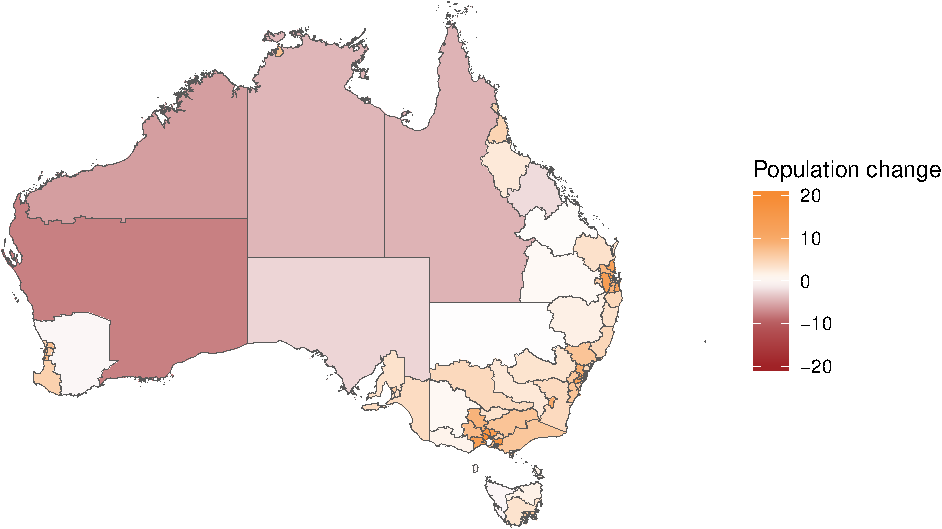
\includegraphics{Data_visualisation_files/figure-latex/map1-1.pdf}

\hypertarget{creating-simple-interactive-graphs-with-plotly}{%
\section{\texorpdfstring{Creating simple interactive graphs with \texttt{plotly}}{Creating simple interactive graphs with plotly}}\label{creating-simple-interactive-graphs-with-plotly}}

\texttt{plotly::ggplotly()}

\hypertarget{bin-generate-data-used-before-prior-sections-are-constructed}{%
\section{bin: generate data used (before prior sections are constructed)}\label{bin-generate-data-used-before-prior-sections-are-constructed}}

\begin{Shaded}
\begin{Highlighting}[]
\KeywordTok{library}\NormalTok{(tidyverse)}
\KeywordTok{library}\NormalTok{(janitor)}
\KeywordTok{library}\NormalTok{(absmapsdata)}

\NormalTok{data <-}\StringTok{ }\KeywordTok{read_csv}\NormalTok{(}\StringTok{"data/ABS_REGIONAL_ASGS2016_02082019164509969.csv"}\NormalTok{) }\OperatorTok\StringTok{ }
\StringTok{        }\KeywordTok{clean_names}\NormalTok{() }\OperatorTok\StringTok{ }
\StringTok{        }\KeywordTok{select}\NormalTok{(}\DataTypeTok{data_code =}\NormalTok{ measure,}
\NormalTok{               data_item,}
               \DataTypeTok{asgs =}\NormalTok{ regiontype,}
               \DataTypeTok{sa4_code_2016 =}\NormalTok{ asgs_}\DecValTok{2016}\NormalTok{,}
               \DataTypeTok{sa4_name_2016 =}\NormalTok{ region,}
               \DataTypeTok{year =}\NormalTok{ time,}
\NormalTok{               value) }\OperatorTok\StringTok{ }
\StringTok{        }\KeywordTok{mutate}\NormalTok{(}\DataTypeTok{sa4_code_2016 =} \KeywordTok{as.character}\NormalTok{(sa4_code_}\DecValTok{2016}\NormalTok{)) }\OperatorTok\StringTok{ }
\StringTok{        }\KeywordTok{left_join}\NormalTok{(sa42016 }\OperatorTok\StringTok{ }\KeywordTok{select}\NormalTok{(sa4_code_}\DecValTok{2016}\NormalTok{, state_name_}\DecValTok{2016}\NormalTok{)) }\OperatorTok\StringTok{ }
\StringTok{        }\KeywordTok{rename}\NormalTok{(}\DataTypeTok{state =}\NormalTok{ state_name_}\DecValTok{2016}\NormalTok{,}
               \DataTypeTok{sa4_code =}\NormalTok{ sa4_code_}\DecValTok{2016}\NormalTok{,}
               \DataTypeTok{sa4_name =}\NormalTok{ sa4_name_}\DecValTok{2016}\NormalTok{) }\OperatorTok\StringTok{ }
\StringTok{        }\KeywordTok{mutate}\NormalTok{(}\DataTypeTok{state_long =}\NormalTok{ state,}
               \DataTypeTok{state =}\NormalTok{ strayr}\OperatorTok{::}\KeywordTok{strayr}\NormalTok{(state_long))}
               
\KeywordTok{write_csv}\NormalTok{(data, }\StringTok{"data/population_sa4.csv"}\NormalTok{)}
\end{Highlighting}
\end{Shaded}

\hypertarget{reading-data}{%
\chapter{Reading data}\label{reading-data}}

\hypertarget{importing-data}{%
\section{Importing data}\label{importing-data}}

\hypertarget{reading-csv-files}{%
\subsection{Reading CSV files}\label{reading-csv-files}}

\hypertarget{read_csv}{%
\subsubsection{\texorpdfstring{\texttt{read\_csv()}}{read\_csv()}}\label{read_csv}}

The \texttt{read\_csv()} function from the \texttt{tidyverse} is quicker and smarter than \texttt{read.csv} in base R.

Pitfalls:
1. read\_csv is quicker because it surveys a sample of the data

We can also compress \texttt{.csv} files into \texttt{.zip} files and read them \emph{directly} using \texttt{read\_csv()}:

\begin{Shaded}
\begin{Highlighting}[]
\KeywordTok{read_csv}\NormalTok{(}\StringTok{"data/my_data.zip"}\NormalTok{)}
\end{Highlighting}
\end{Shaded}

This is useful for two reasons:

\begin{enumerate}
\def\labelenumi{\arabic{enumi}.}
\tightlist
\item
  The data takes up less room on your computer; and
\item
  The original data, which shouldn't ever be directly edited, is protected and cannot be directly edited.
\end{enumerate}

\hypertarget{data.tablefread}{%
\subsubsection{\texorpdfstring{\texttt{data.table::fread()}}{data.table::fread()}}\label{data.tablefread}}

The \texttt{fread} function from \texttt{data.table} is quicker than both \texttt{read.csv} and \texttt{read\_csv}.

\hypertarget{readxlread_excel}{%
\subsection{\texorpdfstring{\texttt{readxl::read\_excel()}}{readxl::read\_excel()}}\label{readxlread_excel}}

\hypertarget{rio}{%
\subsection{\texorpdfstring{\texttt{rio}}{rio}}\label{rio}}

\hypertarget{readabs}{%
\subsection{\texorpdfstring{\texttt{readabs}}{readabs}}\label{readabs}}

\hypertarget{reading-common-files}{%
\section{Reading common files:}\label{reading-common-files}}

\begin{itemize}
\tightlist
\item
  TableBuilder CSVSTRINGs
\item
  HES household file
\item
  SIH
\item
  LSAY and derivatives
\end{itemize}

See data directory for a list of microdata available to Grattan.

\hypertarget{appropriately-renaming-variables}{%
\section{Appropriately renaming variables}\label{appropriately-renaming-variables}}

As shown in the style guide

Add \texttt{rename\_abs} function to a common Grattan package?

\hypertarget{getting-to-tidy-data}{%
\section{Getting to tidy data}\label{getting-to-tidy-data}}

\texttt{pivot\_long()} and \texttt{pivot\_wide()}
\emph{Make sure these are stable btw}

\hypertarget{different-data-types}{%
\chapter{Different data types}\label{different-data-types}}

\hypertarget{tidy-data}{%
\section{Tidy data}\label{tidy-data}}

Other data structures

\hypertarget{dates-with-lubridate}{%
\section{\texorpdfstring{Dates with \texttt{lubridate::}}{Dates with lubridate::}}\label{dates-with-lubridate}}

The \texttt{lubridate::} package

\hypertarget{strings-with-stringr}{%
\section{\texorpdfstring{Strings with \texttt{stringr::}}{Strings with stringr::}}\label{strings-with-stringr}}

\begin{itemize}
\tightlist
\item
  Replacing values
\item
  Matching values
\item
  Separating columns
\end{itemize}

\hypertarget{factors-with-forcats}{%
\section{\texorpdfstring{Factors with \texttt{forcats::}}{Factors with forcats::}}\label{factors-with-forcats}}

\begin{itemize}
\tightlist
\item
  Dangers with factors
\end{itemize}

\hypertarget{data-transformation}{%
\chapter{Data transformation}\label{data-transformation}}

\hypertarget{the-pipe}{%
\section{The pipe}\label{the-pipe}}

\hypertarget{key-dplyr-functions}{%
\section{\texorpdfstring{Key \texttt{dplyr} functions:}{Key dplyr functions:}}\label{key-dplyr-functions}}

All have the same syntax structure, which enable pipe-chains.

\hypertarget{filter-with-filter}{%
\section{\texorpdfstring{Filter with \texttt{filter()}}{Filter with filter()}}\label{filter-with-filter}}

\hypertarget{arrange-with-arrange}{%
\section{\texorpdfstring{Arrange with \texttt{arrange()}}{Arrange with arrange()}}\label{arrange-with-arrange}}

\hypertarget{select-variables-with-select}{%
\section{\texorpdfstring{Select variables with \texttt{select()}}{Select variables with select()}}\label{select-variables-with-select}}

\hypertarget{group-data-with-group_by}{%
\section{\texorpdfstring{Group data with \texttt{group\_by()}}{Group data with group\_by()}}\label{group-data-with-group_by}}

\hypertarget{edit-and-add-new-variables-with-mutate}{%
\section{\texorpdfstring{Edit and add new variables with \texttt{mutate()}}{Edit and add new variables with mutate()}}\label{edit-and-add-new-variables-with-mutate}}

\hypertarget{cases-when-you-should-use-case_when}{%
\subsection{\texorpdfstring{Cases when you should use \texttt{case\_when()}}{Cases when you should use case\_when()}}\label{cases-when-you-should-use-case_when}}

\hypertarget{summarise-data-with-summarise}{%
\section{\texorpdfstring{Summarise data with \texttt{summarise()}}{Summarise data with summarise()}}\label{summarise-data-with-summarise}}

\hypertarget{joining-datasets-with-_join}{%
\section{\texorpdfstring{Joining datasets with \texttt{*\_join()}}{Joining datasets with *\_join()}}\label{joining-datasets-with-_join}}

\hypertarget{analysis}{%
\chapter{Analysis}\label{analysis}}

\hypertarget{creating-functions}{%
\chapter{Creating functions}\label{creating-functions}}

\hypertarget{it-can-be-useful-to-make-your-own-function}{%
\section{It can be useful to make your own function}\label{it-can-be-useful-to-make-your-own-function}}

Why on earth would you create your own function?

\hypertarget{defining-simple-functions}{%
\section{Defining simple functions}\label{defining-simple-functions}}

\hypertarget{more-complex-functions}{%
\section{More complex functions}\label{more-complex-functions}}

\hypertarget{sets-of-functions}{%
\section{Sets of functions}\label{sets-of-functions}}

\hypertarget{using-purrrmap}{%
\section{\texorpdfstring{Using \texttt{purrr::map}}{Using purrr::map}}\label{using-purrrmap}}

\hypertarget{sharing-your-useful-functions-with-grattan}{%
\section{Sharing your useful functions with Grattan}\label{sharing-your-useful-functions-with-grattan}}

\hypertarget{version-control}{%
\chapter{Version control}\label{version-control}}

\hypertarget{version-control-is-important-and-intimidating}{%
\section{Version control is important and intimidating}\label{version-control-is-important-and-intimidating}}

Version control is great!

\hypertarget{github}{%
\section{Github}\label{github}}

We use Github to version-control and share reports in LaTeX, so you're already a bit set-up.

\hypertarget{git}{%
\section{Git}\label{git}}

Using Git within R Studio\ldots{}

\bibliography{book.bib,packages.bib}


\end{document}
